\documentclass[a4,12pt]{report}
\usepackage[T1]{fontenc}
\usepackage{textcomp}
\usepackage[utf8]{inputenc}
\usepackage[russian]{babel}
\usepackage{graphics}
\usepackage{graphicx}
\usepackage{epstopdf}
\usepackage{amsmath}
\usepackage{hyperref}
\usepackage{fancyvrb}
\usepackage{verbatim}
\usepackage{cmap}
%\renewcommand{\familydefault}{\sfdefault}
\textwidth=16cm
\oddsidemargin=0.1cm
\linespread{1.2}

\newcommand{\HRule}{\rule{\linewidth}{0.5mm}}
\DefineVerbatimEnvironment{code}{Verbatim}{frame=single, fontsize=\small}

\begin{document}

\begin{titlepage}

\begin{center}

\begin{tabular}{ l @{\hspace{1.2cm}}r }

\includegraphics[scale=0.3]{rhm.jpg} & 
\includegraphics[scale=0.9]{sibnigmi.jpg}\\[3cm]
\end{tabular}

% Title
\HRule \\[0.4cm]
{ \huge \bfseries Система генерации GPU-кода для модели COSMO}\\[0.4cm]

\HRule \\[0.5cm]

\textsc{\Large отчёт по этапу I}\\[1.5cm]


% Author and supervisor
\begin{minipage}{0.4\textwidth}
\begin{flushleft} \large
Д.~Н.~Микушин \\
{\small maemarcus@gmail.com} \\[0.5cm]
А.~А.~Мыльцев \\
{\small alexander.myltsev@gmail.com}
\end{flushleft}
\end{minipage}
\begin{minipage}{0.4\textwidth}
\begin{flushright} \large
А.~П.~Петров \\
{\small artem.petrov80@gmail.com} \\[0.5cm]
Ю.~В.~Мартынова \\
{\small foxyj13@gmail.com} \\[0.5cm]
М.~Штемберг \\
{\small warchild1000@mail.ru}
\end{flushright}
\end{minipage}

\vfill

% Bottom of the page
{\large \today}

\end{center}

\end{titlepage}

\tableofcontents

\begin{abstract}
Работа представляет собой описание совместной деятельности СибНИГМИ и NVIDIA по созданию и внедрению технологий использования GPU в оперативных моделях прогноза погоды. По материалам приоритетного проекта POMPA дана характеристика вычислительных аспектов модели COSMO. На основе анализа других работ последовательно выстраивается аргументация для создания системы преобразования исходного кода с оптимальными свойствами. Реализуемый метод генерации GPU-ядер без изменения исходного кода модели по-видимому является наиболее мягким и консервативным из всех возможных решений с точки зрения пользователя и наиболее трудоёмким с точки зрения разработчика. Приведены результаты первого этапа работы, обзор похожих решений, детали реализации, краткое руководство пользователя и разработчика, предложен план дальнейшего развития системы.
\end{abstract}

\chapter{Краткое описание проекта}

\section{Цель работы}

Цель данной работы состоит в поэтапной разработке метода использования GPU в коде численных моделей на языке Fortran, настроенного на наилучшую поддержку используемых моделей. Предполагается, что метод может занять в настоящее время пустующую нишу средства обеспечения максимально плавного перехода к использованию GPU в программах для языка Fortran. Для этого в первую очередь требуется, чтобы исходный код пользователя по умолчанию компилировался для GPU \textbf{в оригинальном виде}, а необходимость учета факторов, требующих от пользователя специфических знаний о программировании GPU возникала \textbf{только по его желанию}. Важно обеспечить достаточную эффективность расчетов на GPU и высокое качество результатов, что имеет особую важность для оперативных моделей прогноза погоды.

\section{Метод}

Для использования GPU в модели COSMO применен метод автоматической генерации GPU-кода на базе готовых технологий GNU Compiler Toolchain, XSLT, LLVM и NVIDIA CUDA Toolkit. Специально для этой задачи разработан метод автоматического расщепления исходного кода на языке Fortran на части для исполнения на GPU и CPU, включающий транслятор вида Fortran95 $\rightarrow$ Fortran95 $\rightarrow$ Fortran95 $+$ CUDA C и runtime-библиотеку. Библиотека реализует функции запуска ядер и синхронизации данных между GPU и CPU с учетом косвенных зависимостей, таких как данные в модулях. Функции также реализуют специальный режим контрольного расчета, при котором все вычисления производятся одновременно на CPU и GPU с проверкой на условие предельного уровня расхождения результатов для каждого отдельного ядра.

\section{Этапы работы}

Цель проекта предполагается достигнуть в два этапа:
\begin{enumerate}
\item реализация общей схемы, тестирование, проверка правильности результатов модели COSMO (апрель-июнь)
\item вычислительная эффективность, повышение доли параллельных циклов, использующих GPU (июль-сентябрь)
\end{enumerate}
На первом этапе должна быть подготовлена и реализована структурная схема компилятора, состоящая как из готовых компонентов, так и специально разработанных. Программная оболочка уже должна иметь достаточно завершенный вид для применения конечным пользователем. Необходимо представить убедительные результаты надежной и корректной работы метода в сложных приложениях, что делает оправданным работы по его дальнейшему улучшению и внедрению.

Приоритеты второго этапа --- доля портированных на GPU циклов, производительность вычислительного кода на GPU, эффективность обмена данными. Если результатом первого этапа является надежно работающая модель, то результат второго --- работающая надёжно и быстро. Предполагается, что основные работы могут быть связаны с \emph{выпуклым анализом} (polyhedral analysis) вычислительных циклов, оптимальным позиционированием обменов данными в соответствии с графом зависимостей, использованием shared-памяти в GPU-ядрах.

\section{Основные результаты первого этапа}

Компилятор с генерацией GPU-ядер реализован и может быть использован конечным пользователем. Проведено тестирование модели COSMO в режиме сравнения с контрольными результатами, для подавляющего числа запусков GPU-ядер получены расхождения результатов менее установленного порога $10^{-4}$ для вещественных массивов и точное совпадение результатов для целочисленных величин (рис.~\ref{fig:compare}).

\begin{figure}
\centering
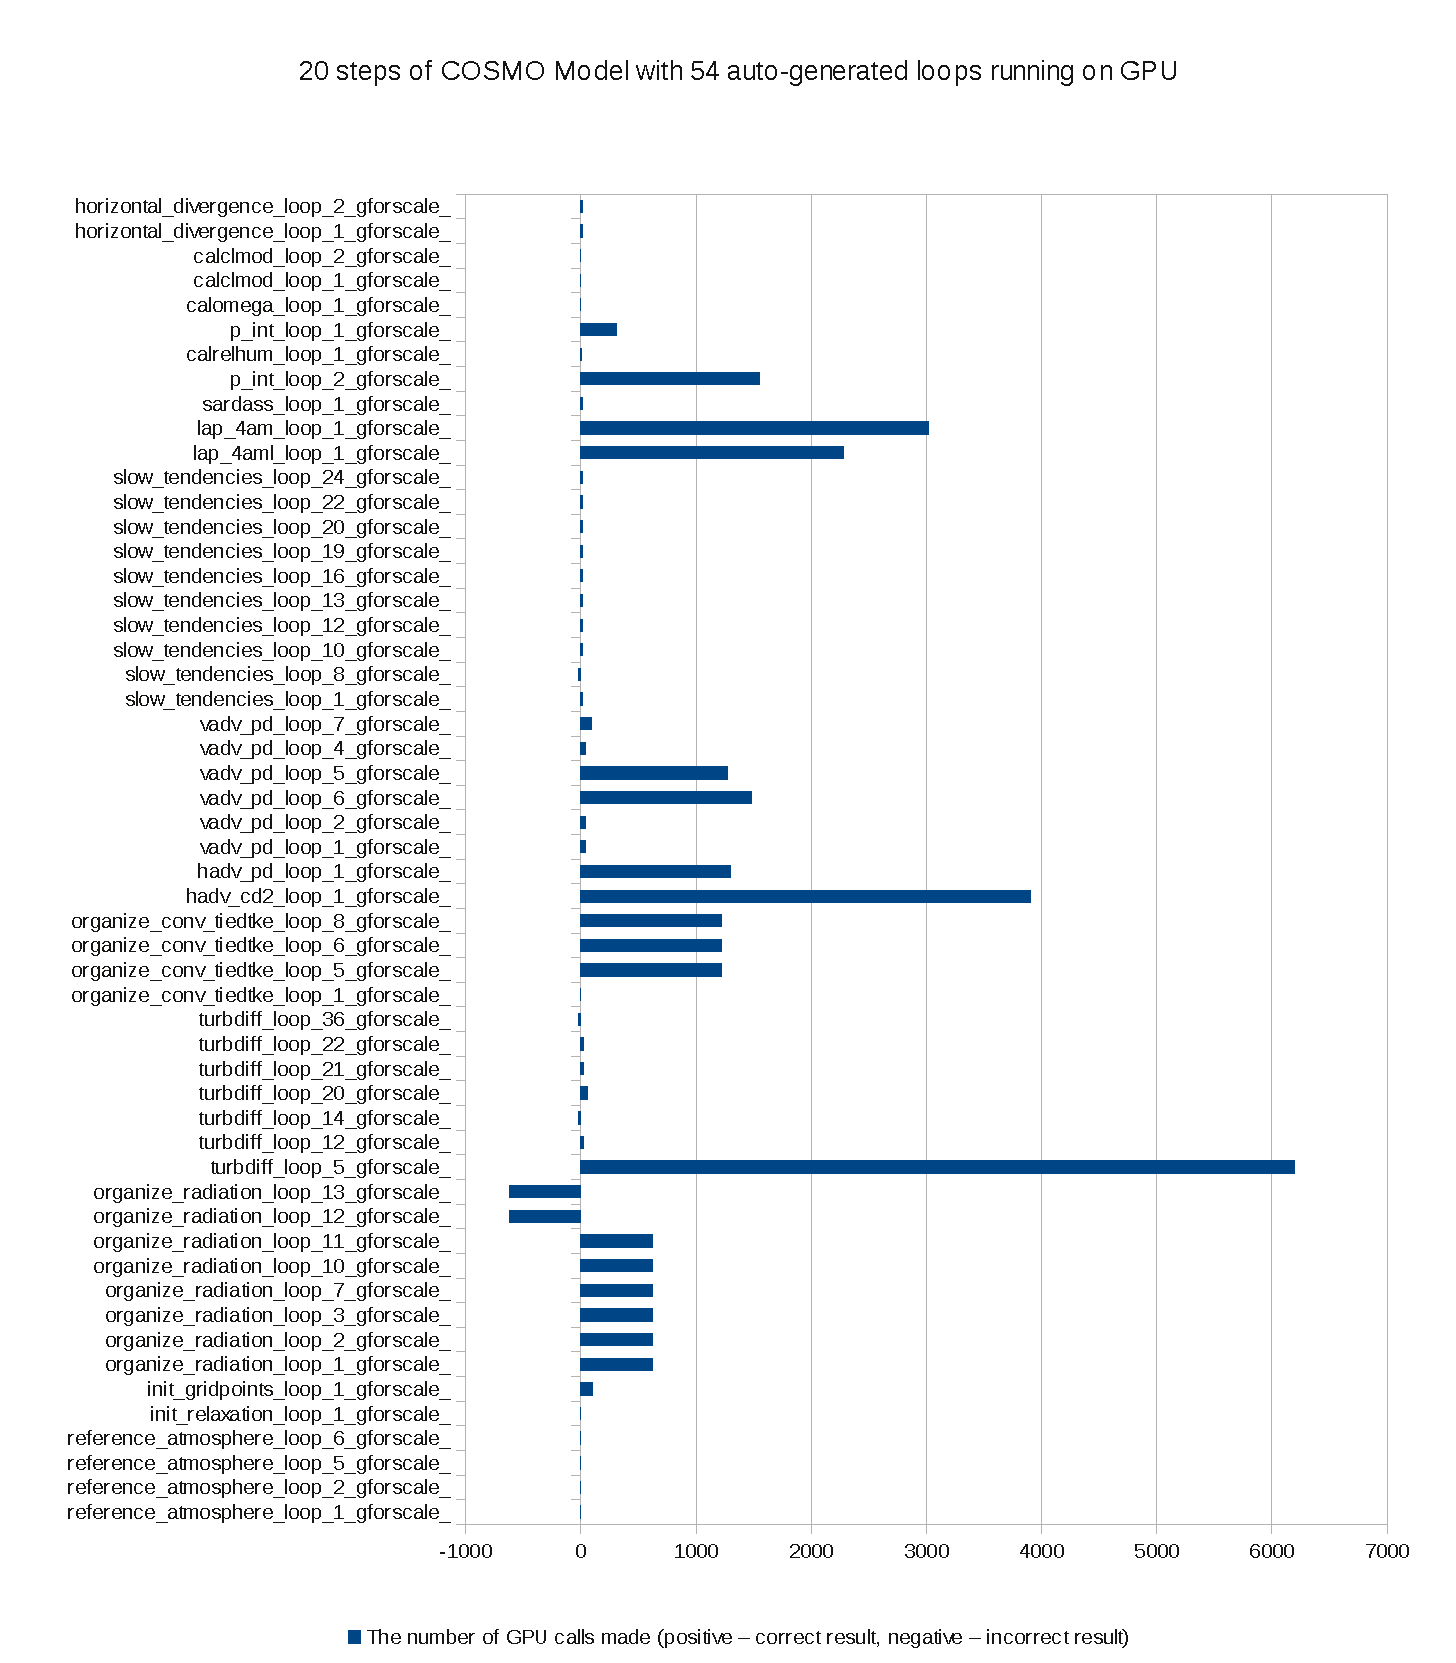
\includegraphics[scale=0.7]{cosmo_20-54_test}
\caption{Тестовый запуск модели COSMO с 54 сгенерированными GPU-ядрами в режиме сравнения результатов}
\label{fig:compare}
\end{figure}

\chapter{Основные сведения о модели COSMO}

Модель COSMO --- региональная разностная модель атмосферы и подстилающей поверхности, используемая в качестве оперативной модели метеослужбами ряда стран Европы и Гидрометцентром РФ. Вычислительное ядро представлено единым приложением с исходным кодом на языке Fortran, около 250 тыс. строк. Распределение вычислений реализуется при помощи двумерной декомпозиции горизонтальной широтно-долготной сетки и интерфейса MPI. Производительность модели составляет 3-13\% пиковой в зависимости от используемой вычислительной системы. Такое значение типично для моделей подобного класса и может быть обусловлено, главным образом, пропускной способностью памяти и коммуникационной сети (рис.~\ref{fig:01}).

Разработчики модели отмечают привлекательные характеристики GPU --- энергоэффективность, большая пропускная способность памяти, меньшая цена. С другой стороны, развитие GPU-реализации сдерживается рядом факторов --- сложностью, затратами на поддержку обратной совместимости и малой выгодой от частичного портирования кода (рис.~\ref{fig:02}). В числе недостатков также отмечена необходимость привязки к закрытой технологии конкретного производителя (рис.~\ref{fig:10}).

\begin{figure}
\centering
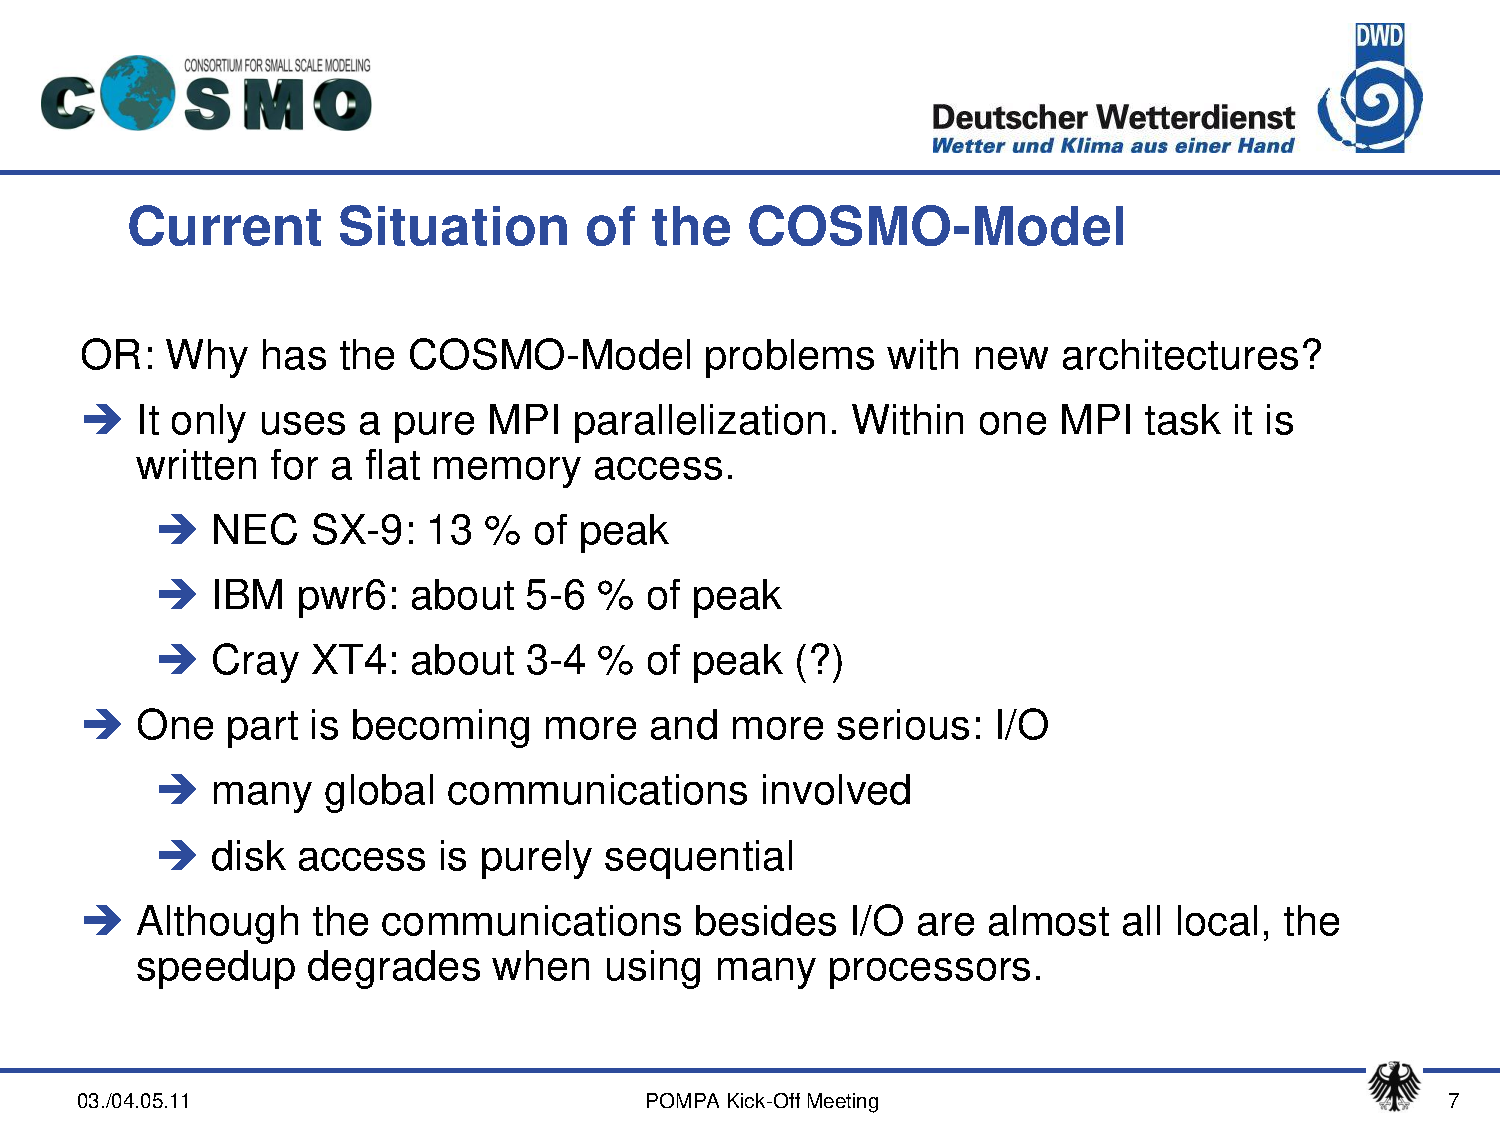
\includegraphics[scale=0.4]{slides/01.pdf}
\caption{Проблемы вычислительной эффективности модели COSMO (Ulrich Schättler)}
\label{fig:01}
\end{figure}

\begin{figure}
\centering
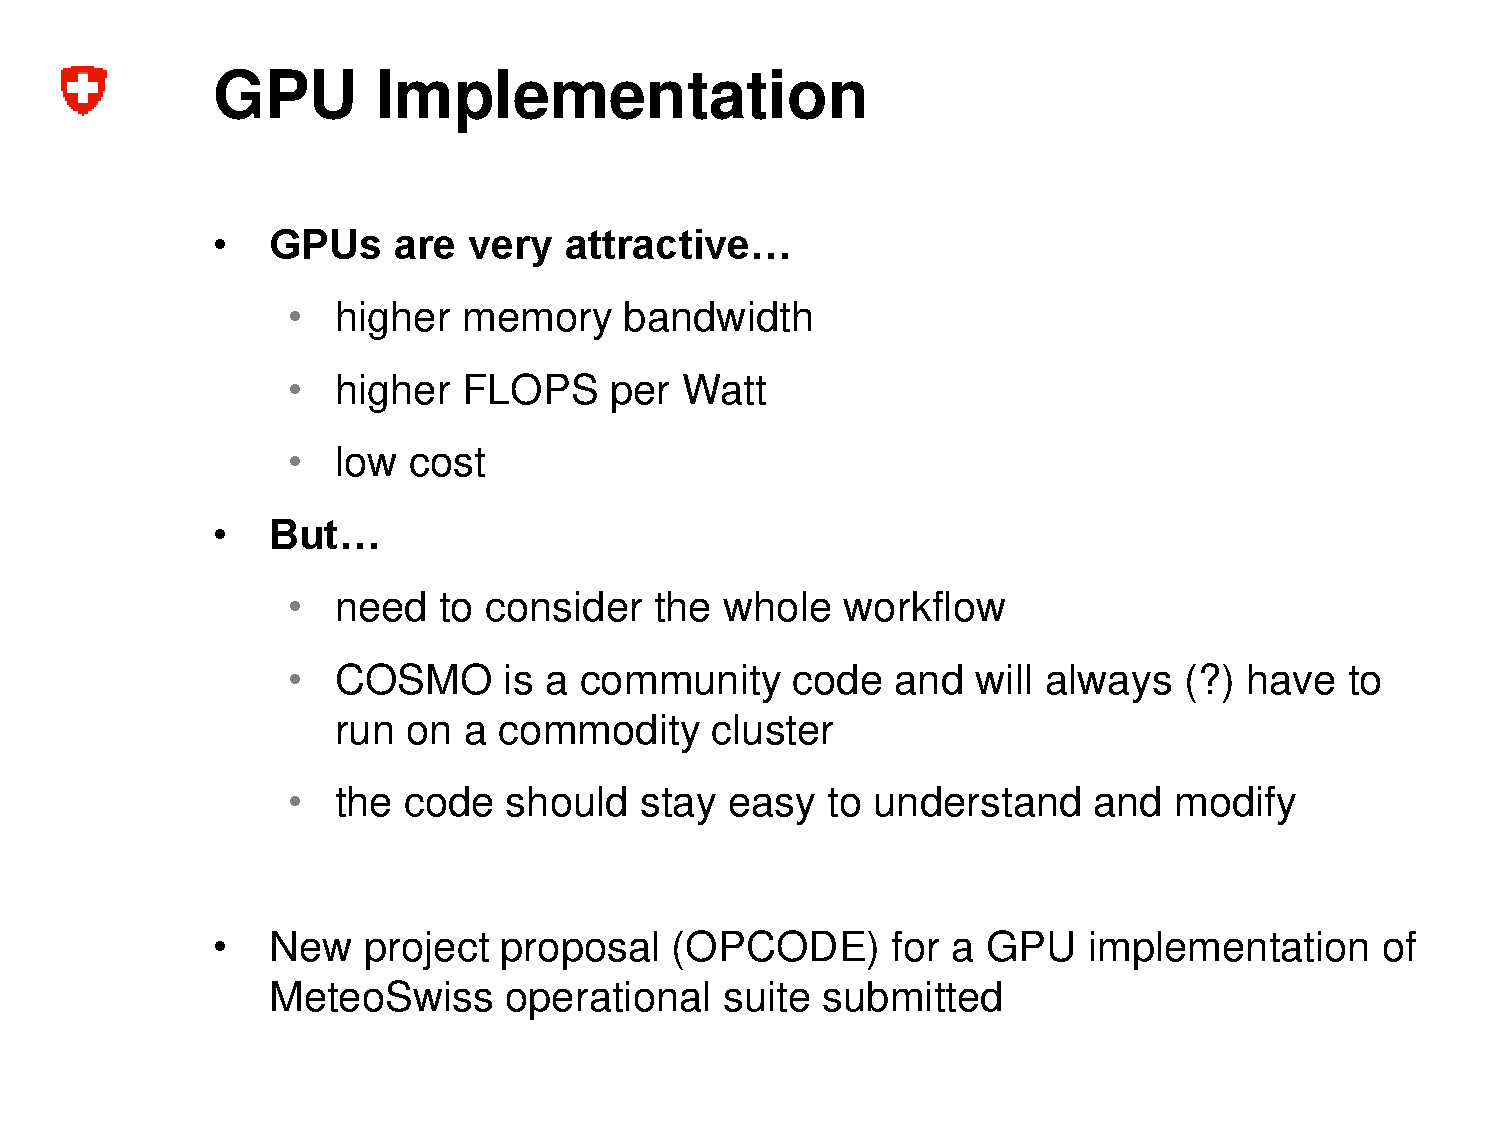
\includegraphics[scale=0.4]{slides/02.pdf}
\caption{Сочетание преимуществ GPU и требований к модели (Oliver Fuhrer)}
\label{fig:02}
\end{figure}


\chapter{Выбор оптимальной программной модели}

Конкретным результатом данной работы должна стать \textbf{востребованная} GPU-версия модели COSMO. Обеспечение востребованности является намного более сложной задачей, чем простое портирование кода на GPU. Например, для LINPACK фактически достаточно получить правильный результат решения стандартной задачи быстрее конкурирующих систем. При этом не так уж и важно, каким образом он достигнут и насколько сложно будет сделать то же самое другим разработчикам по отношению к своим задачам, если они имеют меньше знаний о вычислительной специфике. Работа над COSMO --- это противоположный случай: необходимо учесть интересы пользователей и разработчиков модели, с тем чтобы обеспечить дальнейшее развитие GPU-реализации силами сообщества. Поэтому ориентиром для работы являются идеи, развиваемые в рамках приоритетного проекта POMPA. При выборе направления работы проанализирован ряд перспективных подходов, представленных на POMPA Kick-off Meeting, окончательное решение основано на анализе их преимуществ и недостатков.

\section{PGI CUDA Fortran}

ФФ

\section{PGI Accelerator}

Программная модель PGI Accelerator является системой разметки параллельных циклов, встроенной в язык, подобно OpenMP. В директивах PGI Accelerator указываются зависимые данные вычислительного цикла и, в случае необходимости, режим их пересылки между памятью CPU и GPU (рис.~\ref{fig:06}). Для GPU-ядра, полученного при компиляции цикла с директивой \$acc region, компилятор автоматически выбирает количество рабочих блоков и потоков.


Для блока облачной микрофизики с помощью PGI Accelerator и GPU архитектуры Fermi продемонстрирована возможность получения двукратного прироста производительности по сравнению с 12-ядерным процессором (рис.~\ref{fig:07}). В то же время авторы отмечают большой объём необходимой ручной работы по оптимизации кода, например, по перестановке циклов (впрочем из презентации не ясно, была ли проведена аналогичная перестановка в коде для CPU и не приводит ли она к аналогичному приросту производительности), рис.~\ref{fig:08}.

\begin{figure}
\centering
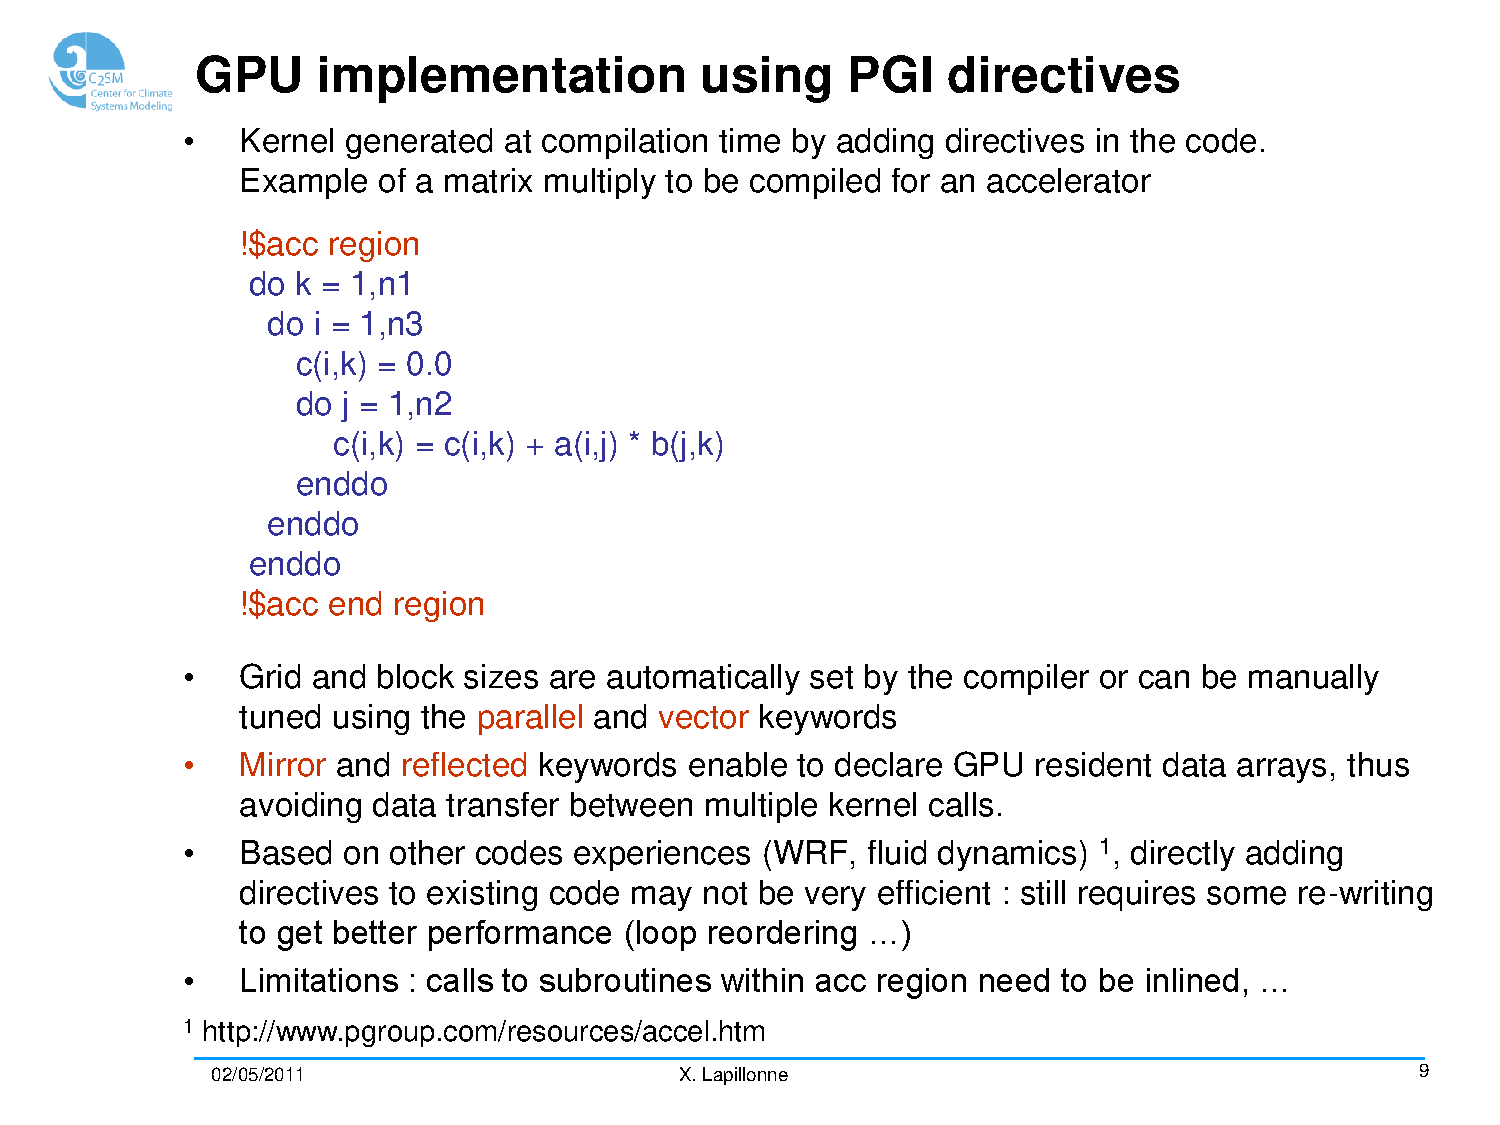
\includegraphics[scale=0.4]{slides/06.pdf}
\caption{Особенности программирования директивами PGI Accelerator (Xavier Lapillonne, Oliver Fuhrer)}
\label{fig:06}
\end{figure}

\begin{figure}
\centering
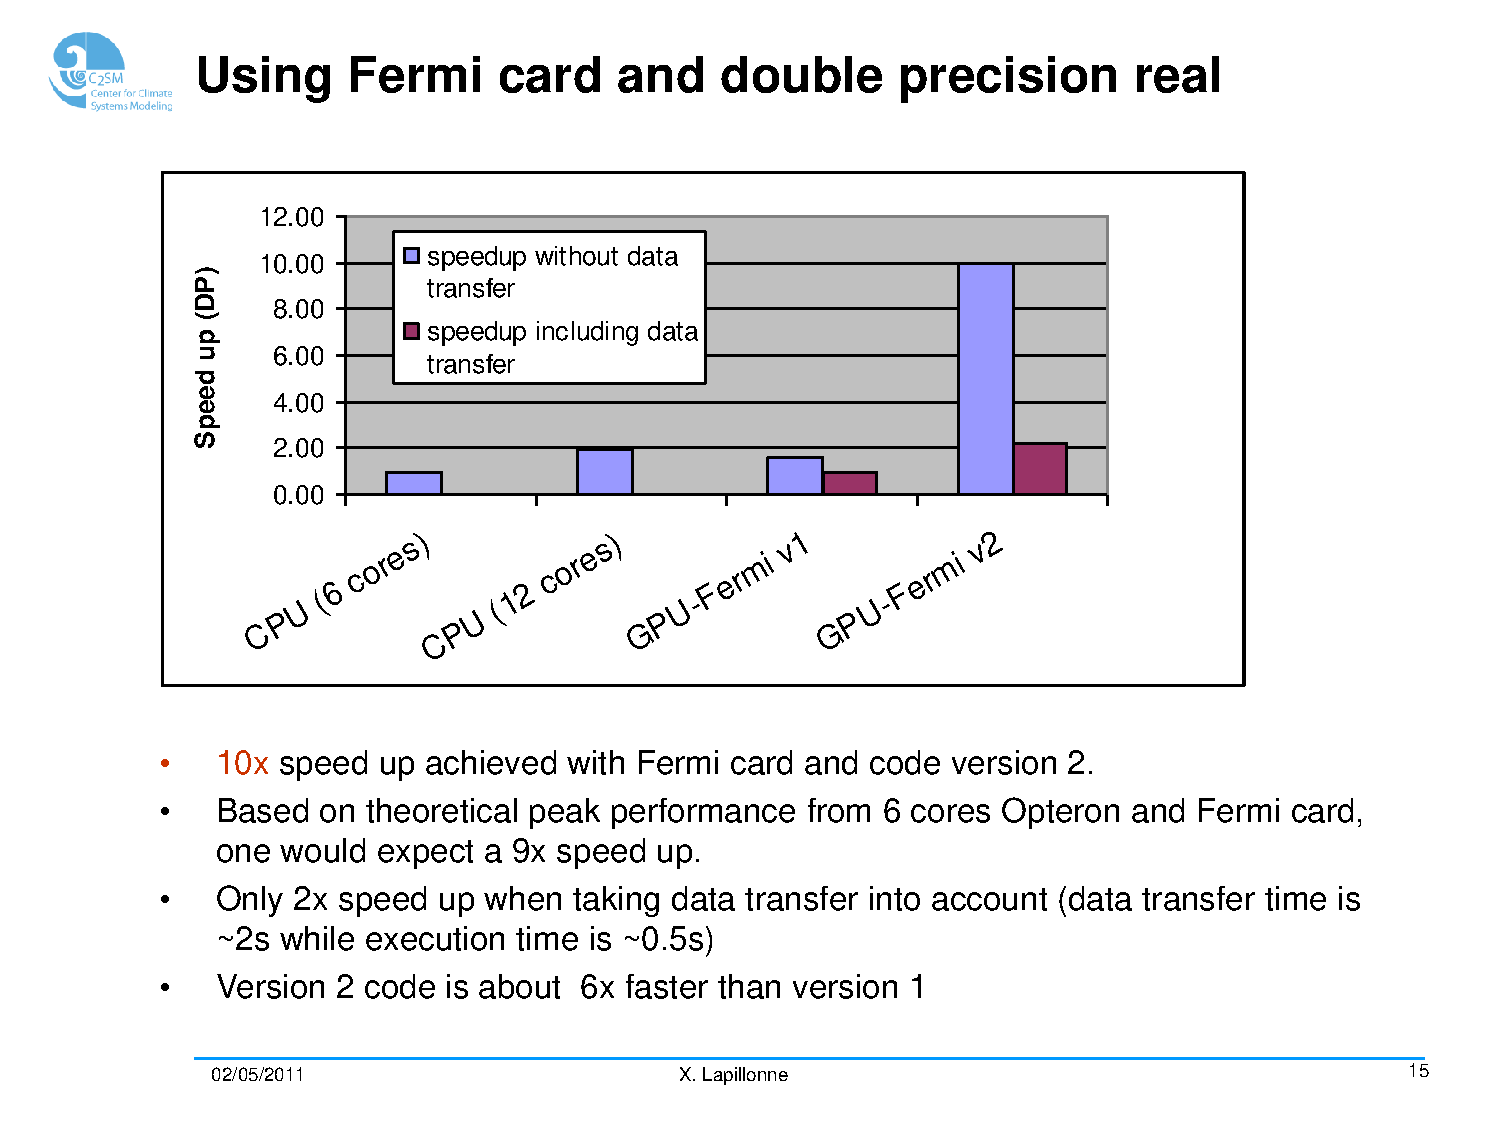
\includegraphics[scale=0.4]{slides/07.pdf}
\caption{Сравнение производительности CPU и PGI Accelerator на примере блока облачной микрофизики (Xavier Lapillonne, Oliver Fuhrer)}
\label{fig:07}
\end{figure}

\section{PathScale HMPP / OpenHMPP}

ФФ

\section{f2c-acc}

Компилятор f2c-acc (Mark Govett et al, NOAA) для маркированных директивами циклов заданного исходного кода на языке Fortran генерирует эквивалентный C/C++ код GPU-ядра и хост-драйвера (копирование данных, запуск ядра и тд). В целом метод выглядит как близкий аналог PGI Accelerator, но без привязки к компиляторам PGI (рис.~\ref{fig:08}-\ref{fig:10}). Даже если поддержка Fortran 95 реализована достаточно хорошо, в отношении f2c-acc справедлив тот же довод, что и для PGI Accelerator: избыточная ручная работа по определению зависимостей и параллельных циклов. В то же время доступность качественного открытого эквивалента повышает привлекательность решения PGI.

\begin{figure}
\centering
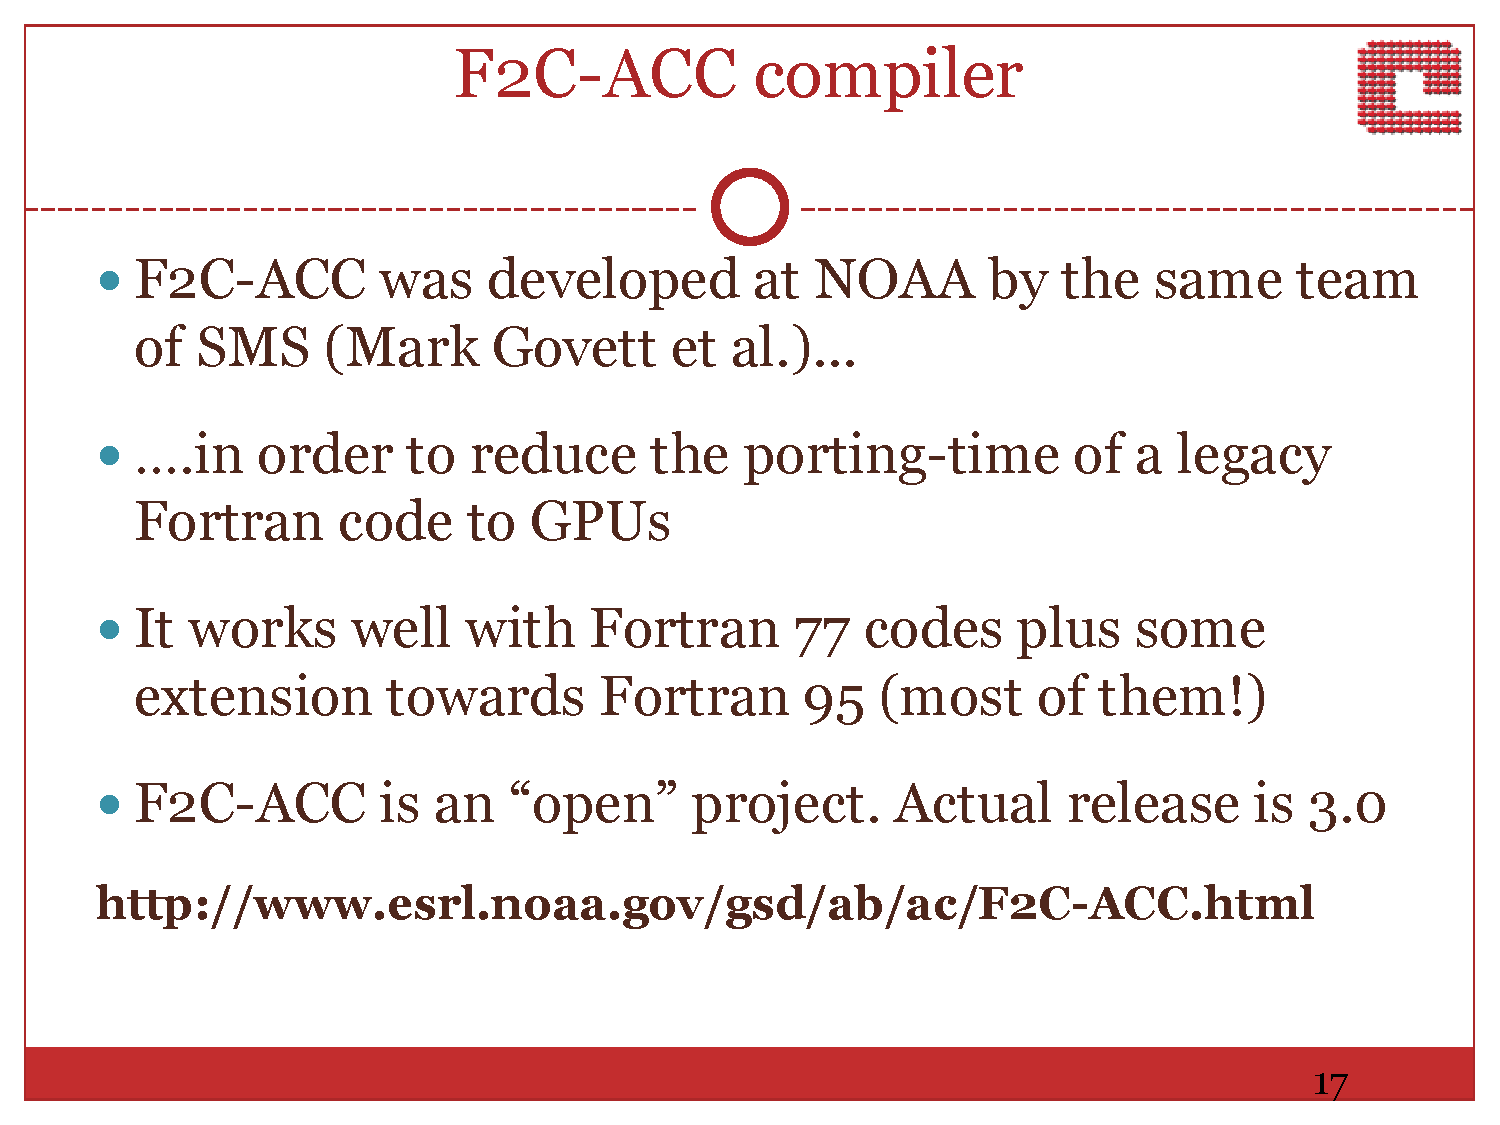
\includegraphics[scale=0.4]{slides/08.pdf}
\caption{Особенности компилятора f2c-acc (Piero Lanucara)}
\label{fig:08}
\end{figure}

\begin{figure}
\centering
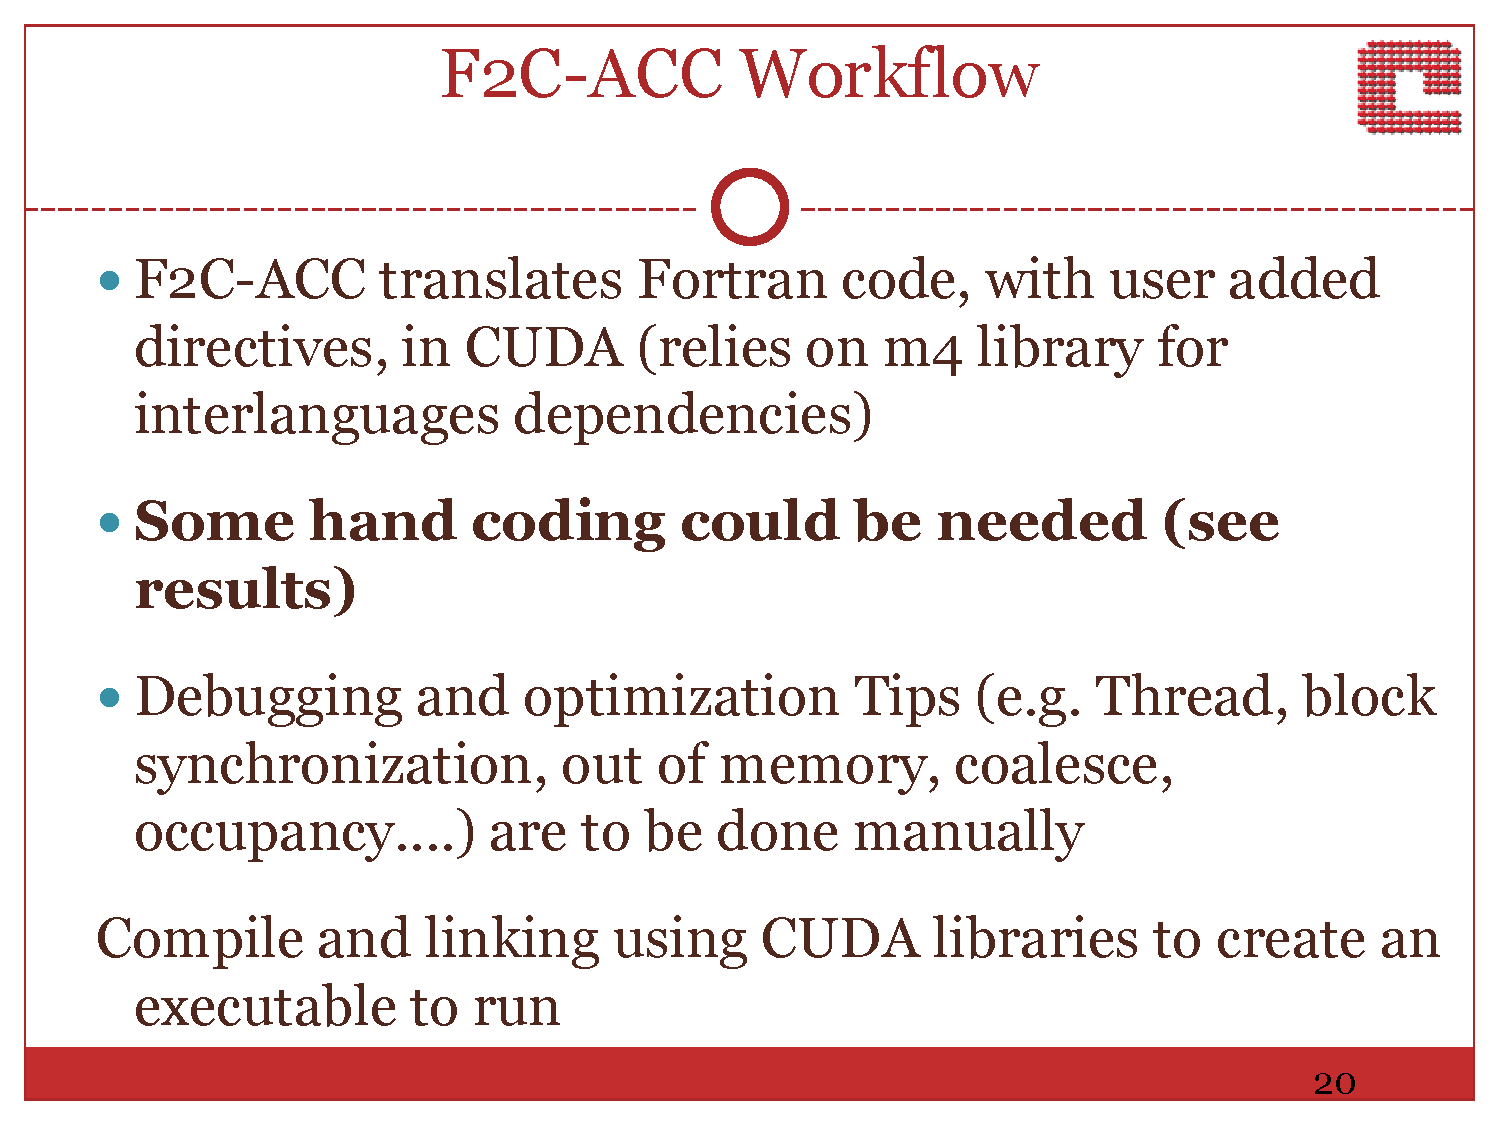
\includegraphics[scale=0.4]{slides/09.pdf}
\caption{Особенности компилятора f2c-acc (Piero Lanucara)}
\label{fig:09}
\end{figure}

\begin{figure}
\centering
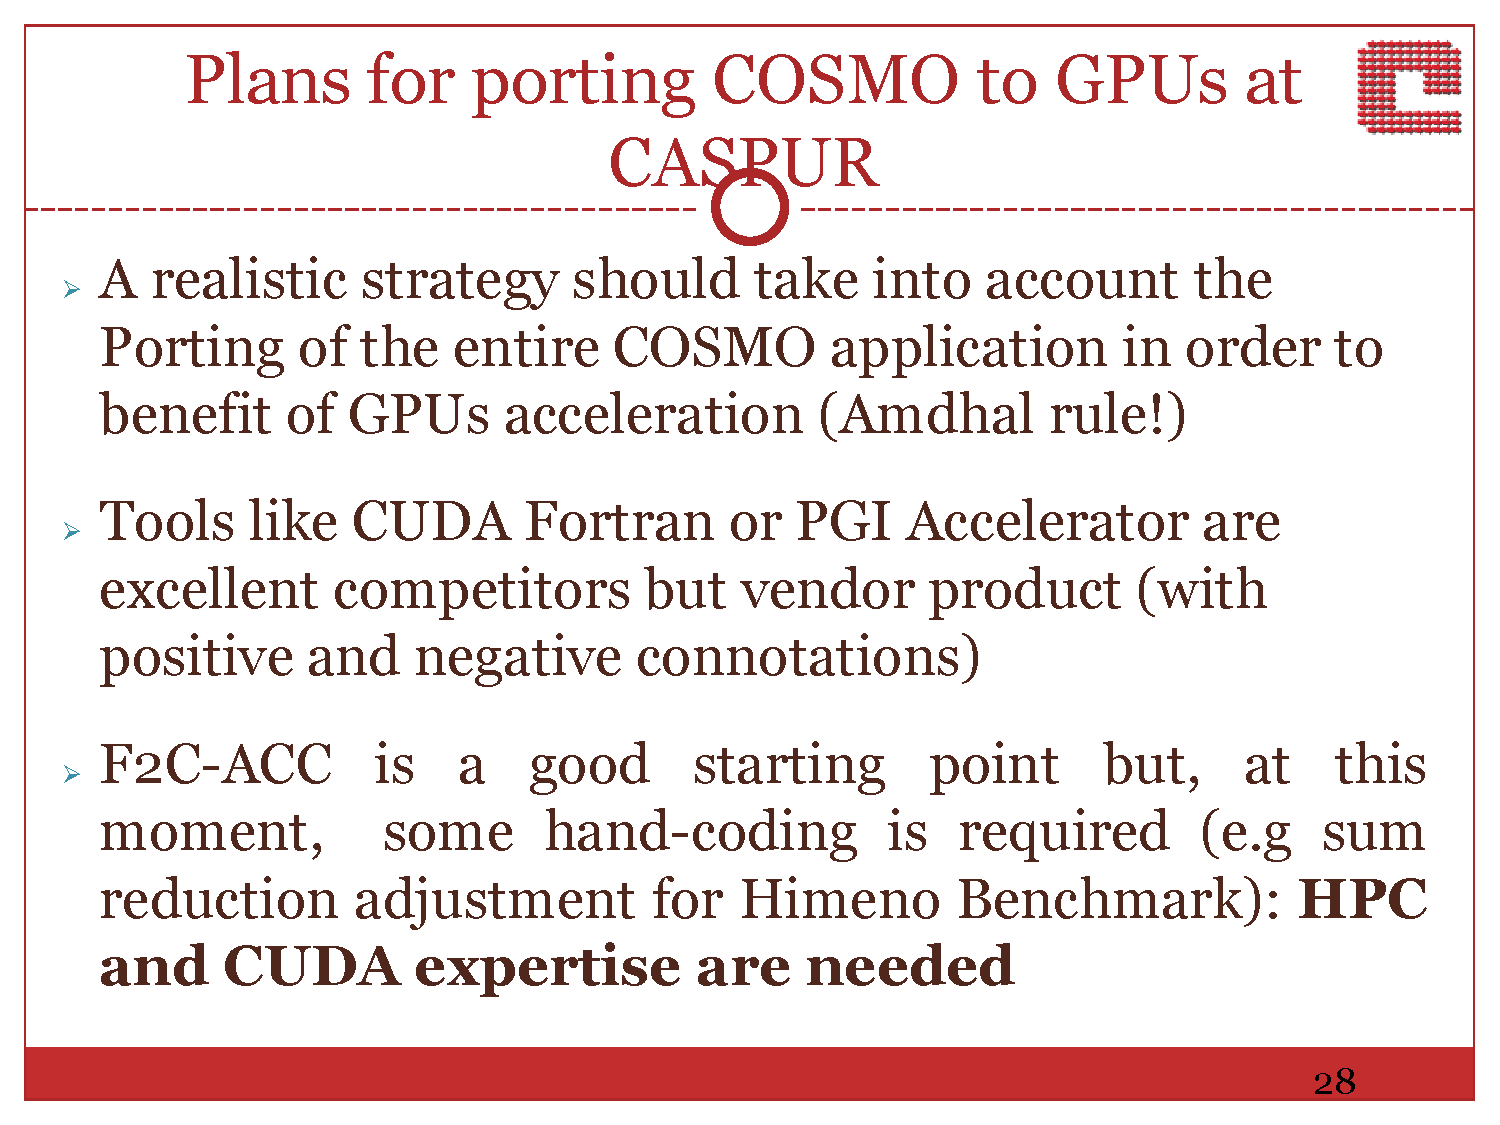
\includegraphics[scale=0.4]{slides/10.pdf}
\caption{Выводы по компилятору f2c-acc (Piero Lanucara)}
\label{fig:10}
\end{figure}

\section{Специализированный язык шаблонов SCS}

Supercomputing Systems AG предлагает ряд оптимизаций для CPU-версии модели COSMO (рис.~\ref{fig:03}):

\begin{itemize}
\item минимизация числа промежуточных массивов (вероятно, в конечном итоге это сводится к уменьшению общего числа хранимых массивов, что теоретически может ослабить зависимость производительности от скорости работы памяти)
\item объединение циклов (вероятно, полезным в действительности может оказаться только объединение циклов, работающих со связанными данными, в противном случае можно ожидать, что положительный эффект будет нивелирован ухудшением кешируемости)
\item наилучший порядок циклов
\end{itemize}

Динамическое ядро модели предполагается переписать на C++ с использованием специализированного API построения разностных схем, что позволит генерировать более эффективный машинный код и в перспективе добавлять различные реализации API, например GPU-бекенд (рис.~\ref{fig:04}-\ref{fig:05}). Очевидно эта задача выполнима: с помощью конструкций подобных STL может быть реализован какой-угодно API и весьма вероятно, что написанный с его помощью код может быть лучше оптимизирован компилятором. С другой стороны неясно, в какой мере такой подход сочетается с необходимостью постоянного развития модели и знаниями её основных разработчиков.

\begin{figure}
\centering
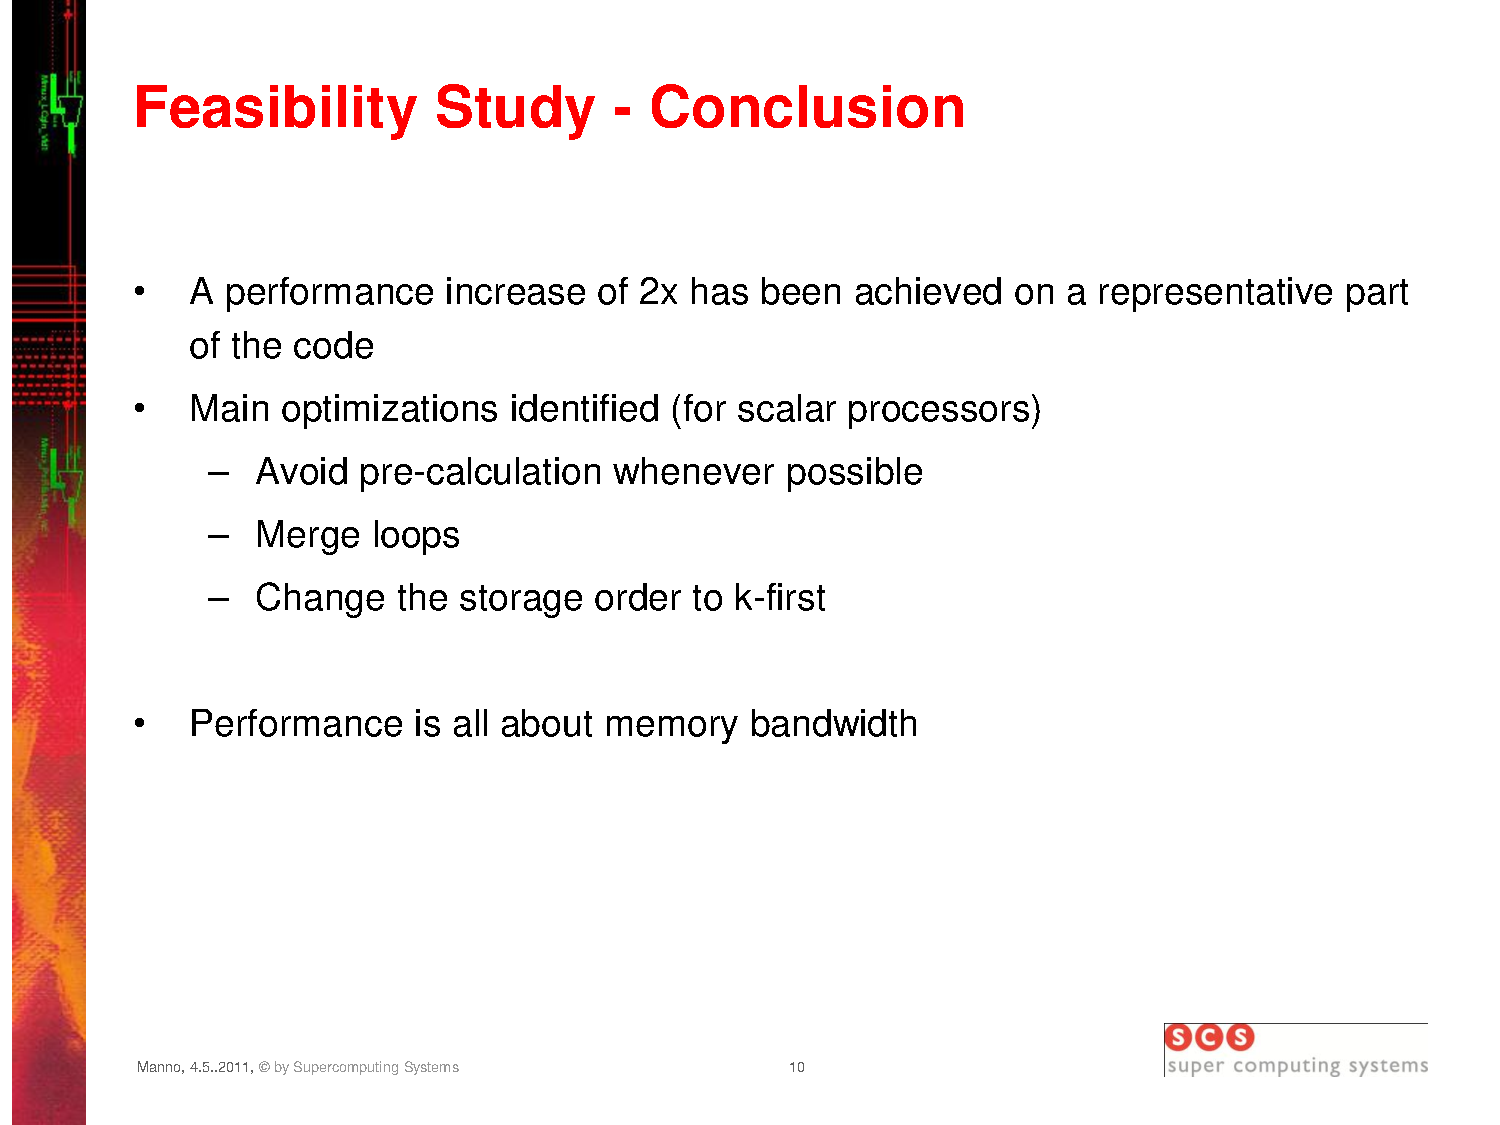
\includegraphics[scale=0.4]{slides/03.pdf}
\caption{Результаты исследования наиболее важных направлений оптимизации исходного кода модели COSMO (Tobias Gysi)}
\label{fig:03}
\end{figure}

\begin{figure}
\centering
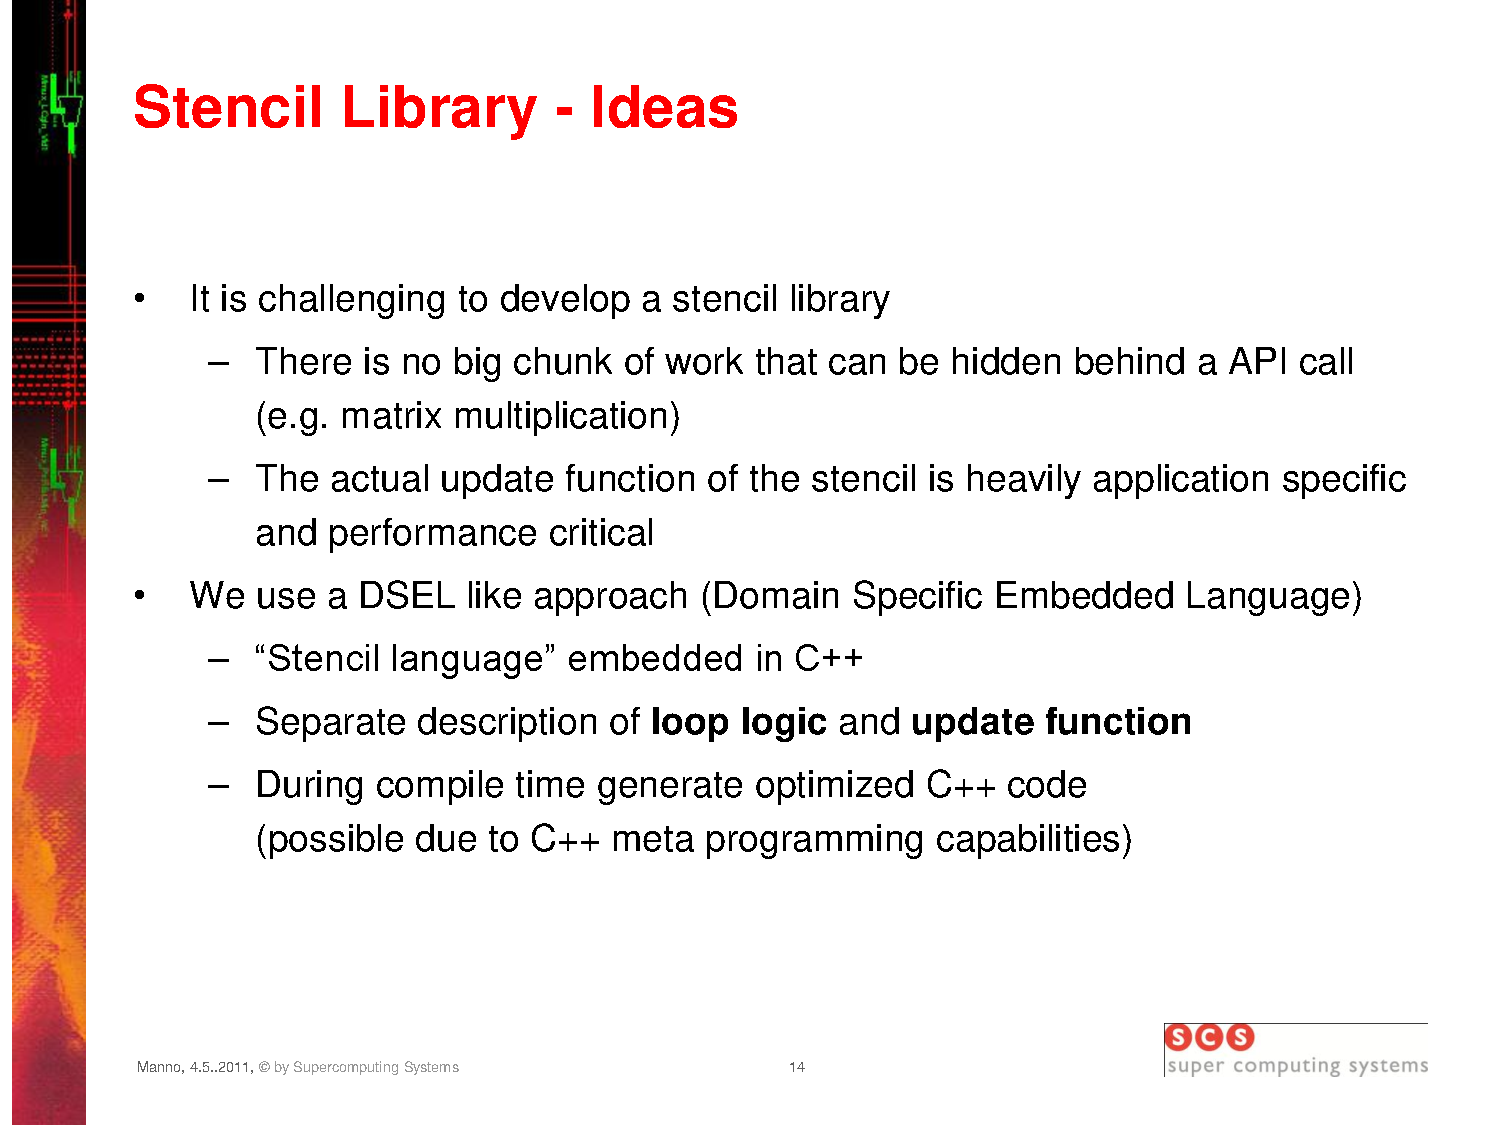
\includegraphics[scale=0.4]{slides/04.pdf}
\caption{Идеи по разработке библиотеки, обобщающей программирование разностных схем (Tobias Gysi)}
\label{fig:04}
\end{figure}

\begin{figure}
\centering
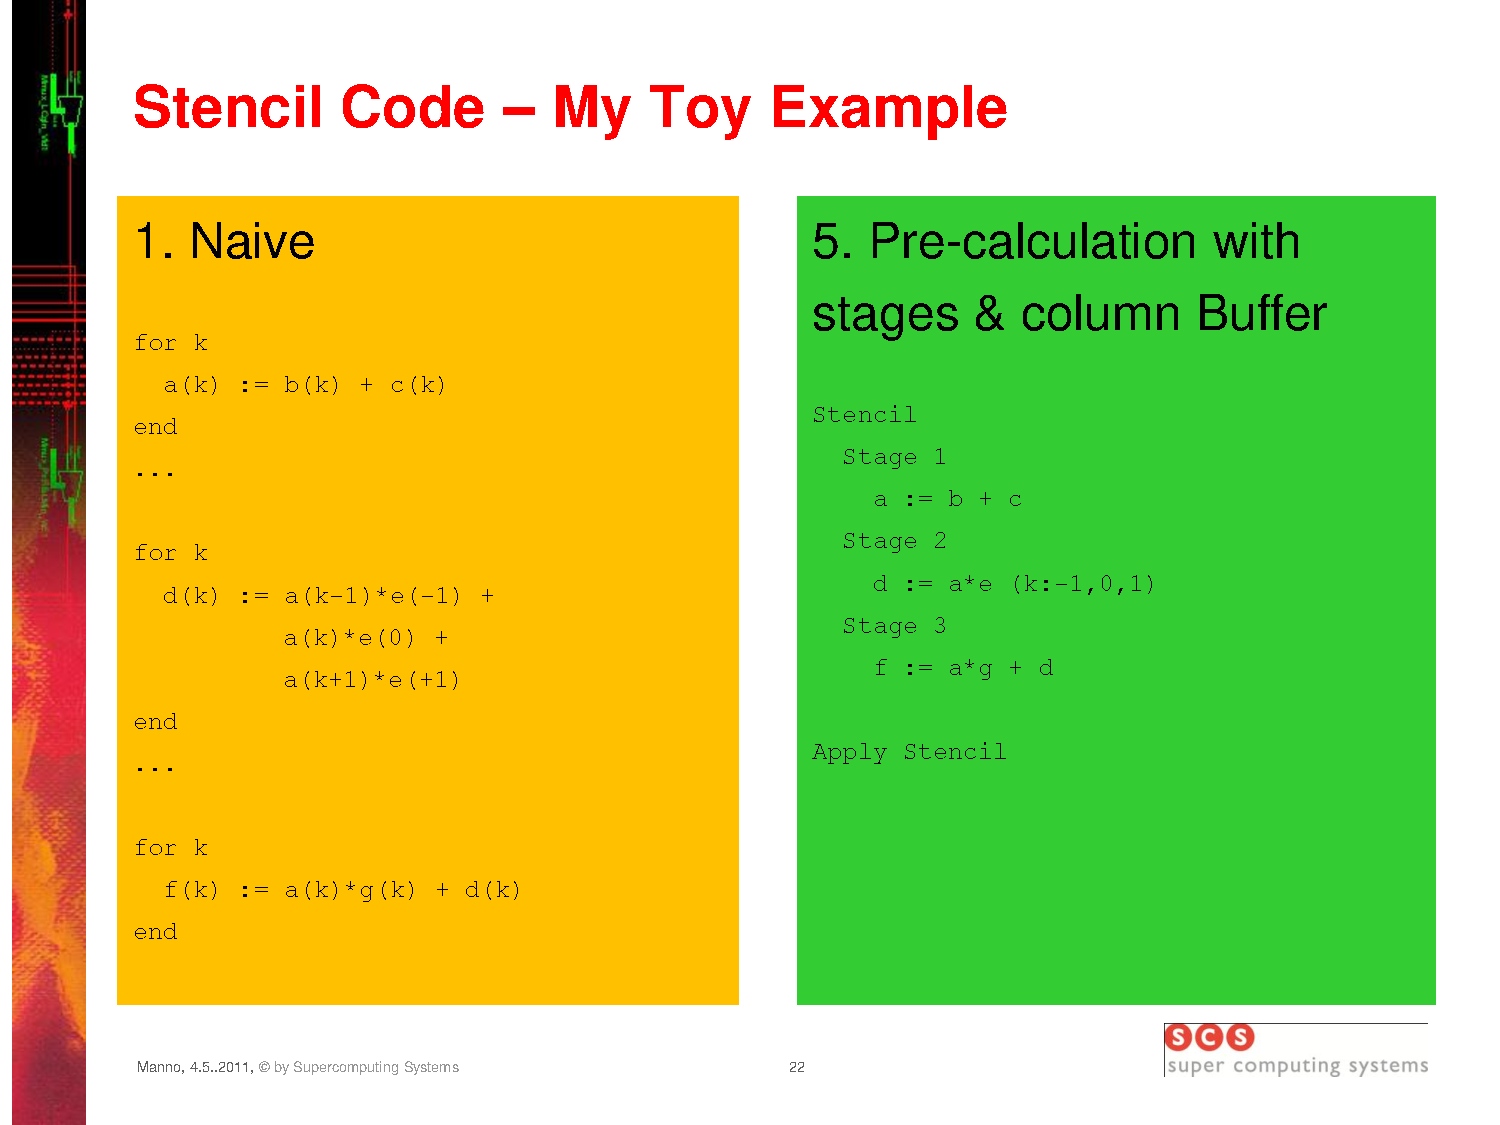
\includegraphics[scale=0.4]{slides/05.pdf}
\caption{Пример использования API построения разностных схем (справа), эквивалентного коду на языке Fortran (слева) (Tobias Gysi)}
\label{fig:05}
\end{figure}


\section{par4all}

ФФ

\section{Обоснование выбора программной модели}

В проектах POMPA и других решениях можно выделить положительные и отрицательные стороны:

\begin{itemize}
\item[\textbf{--}] Все решения требуют, чтобы параллельные циклы были определены пользователем вручную
\item[\textbf{--}] Все решения требуют, чтобы пересылки данных между CPU и GPU были определены пользователем вручную
\item[\textbf{+}] Программные модели, основанные на добавлении директив обеспечивают обратную совместимость
\item[\textbf{--}] Несмотря на то, что компиляция кода для GPU происходит отдельно, коммерческие продукты также привязывают к собственным решениям и компиляцию кода на CPU
\item[\textbf{--}] Коммерческие решения трудно развивать и улучшать, имея доступ только к публичному интерфейсу
\item[\textbf{--}] Единственное открытое решение (f2c-acc) завязано на устаревший компилятор и может требовать значительных ресурсов для обеспечения поддержки современных стандартов языка Fortran
\end{itemize}

Таким образом, наиболее перспективным могло бы оказаться решение со следующими свойствами:

\begin{itemize}
\item Автоматическое выделение параллельных циклов
\item Автоматическое определение зависимостей данных
\item Использование оригинального исходного кода на языке Fortran без каких-либо изменений
\item Возможность подключения любых компиляторов при сборки кода для CPU и GPU
\item Максимально открытое решение, доступное в исходных кодах
\item Использование актуальных разработок с хорошей поддержкой
\item Производительность не хуже, чем у коммерческих решений
\item Возможность проверки правильности результатов работы каждого отдельного GPU-ядра
\end{itemize}

По результатам анализа принято решение реализовать в рамках данной работы систему генерации GPU-кода, удовлетворяющую вышеперечисленным критериям.

\chapter{Система генерации кода для GPU}

ФФ

\section{Трансформация исходного кода}

Ключевой механизм в основе разрабатываемой системы --- расщепление оригинального исходного кода на языке Fortran на части, предназначенные для исполнения на CPU и на GPU и их компиляция. Вообще говоря, не обязательно работать на уровне исходного кода, в некоторых других системах расщепление производится уже во внутреннем представлении компилятора AST (Abstract Syntax Tree). Но в таком случае решение либо жёстко привязывается к компилятору, либо восстанавливает программу из AST для дальнейшей передачи во внешний компилятор. В то же время трансляция кода в AST и генерация из него эквивалентного кода на другом языке является единственным способом решить задачу при отсутствии компилятора Fortran для GPU. Принимая во внимание требования по обеспечению поддержки внешних компиляторов и использованию открытых решений, возможны следующие варианты:

\begin{enumerate}
\item Использование AST открытого компилятора Fortran (например, rose, gfortran, g95 или pathscale) для преобразования исходного кода, поддержка компиляции для CPU и GPU внешними компиляторами
\item Использование AST открытого компилятора Fortran Open64 для преобразования исходного кода, поддержка компиляции для CPU внешним компилятором, компиляция для GPU напрямую из AST с помощью open64-совместимого компилятора nvopencc
\item Использование LLVM, преобразование кода на уровне IR, восстановление эквивалентного кода на C для GPU, компиляция с помощью LLVM или восстановление кода для внешнего компилятора --- для CPU
\item Генерация разметки исходного кода (pretty-printed AST) с помощью открытого компилятора и преобразование его независимыми средствами, например, преобразование XML-разметки исходного кода
\item Использование f2c или f2c-acc для преобразования кода на языке Fortran в C-код.
\end{enumerate}

Первый вариант выглядит наиболее привлекательно в сочетании с gfortran, g95 или pathscale, так как основан на использовании широко поддерживаемых компиляторов (обращаться с rose сложнее, кроме того в нём отсутствует поддержка ряда необходимых возможностей современного стандарта языка Fortran, например, inline-функций). Вместе с тем, развивать его слишком трудно без участия специалистов соответствующего профиля. Возможно, по мере готовности системы и в случае наличия ресурсов, имеет смысл переключиться на этот вариант.


Второй вариант является наиболее дружественным по отношению к средствам, входящим в состав NVIDIA CUDA Toolkit. Теоретически возможно добиться бесшовной компиляции CUDA-кода для GPU в дополнение к преимуществам первого варианта. К сожалению, развивать его бесперспективно, так как nvopencc уже сейчас слабо поддерживается, а в новых выпусках CUDA SDK будет постепенно заменён на nvvm.


Третий вариант делает ставку на LLVM --- проект с коммерчески-совместимой свободной лицензией, имеющий в последние годы исключительный успех. Основная проблема при его использовании --- внутреннее представление наподобие ассемблера (LLVM IR), из-за которого в восстановленном C-коде теряется много высокоуровневой информации, например оригинальный вид циклов. Качество C-backend тем не менее постоянно улучшается. Привлекательная возможность LLVM --- генерация эквивалентного C-кода для любого языка, поддерживаемого GNU-компилятором (C++, Fortran, Ada, Go), что теоретически позволяет перевести на CUDA множество программ.


Четвёртый вариант позволяет получить разбор исходного кода с помощью компонентов компилятора, но при этом работать c простым текстовым представлением AST. К началу проекта по расщеплению кода данным методом уже имелись значительные наработки, использовав которые можно было быстрее всего получить необходимый результат.


Пятый вариант --- f2c --- фактически, надёжно поддерживает только Fortran 77, что не подходит для целевых моделей. Доработка f2c-acc, вероятно, возможна, но требует глубокого анализа.


На первом этапе проекта было принято решение реализовать метод трансформации исходного кода, сочетающий третий и четвёртый вариант: расщепление кода на части для CPU и GPU происходит с помощью разбора исходного кода с XML-разметкой, генерацию CUDA-кода для GPU производит модифицированный LLVM С-backend.

\section{CUDA-backend на основе LLVM}

ФФ

\section{Runtime-библиотека}

ФФ

\section{Общая схема генератора}

Общая схема этапов генерации GPU-кода представлена на рис.~\ref{fig:toolchain_scheme}. Рассмотрим их работу на примере теста axpy.

\begin{figure}
\centering
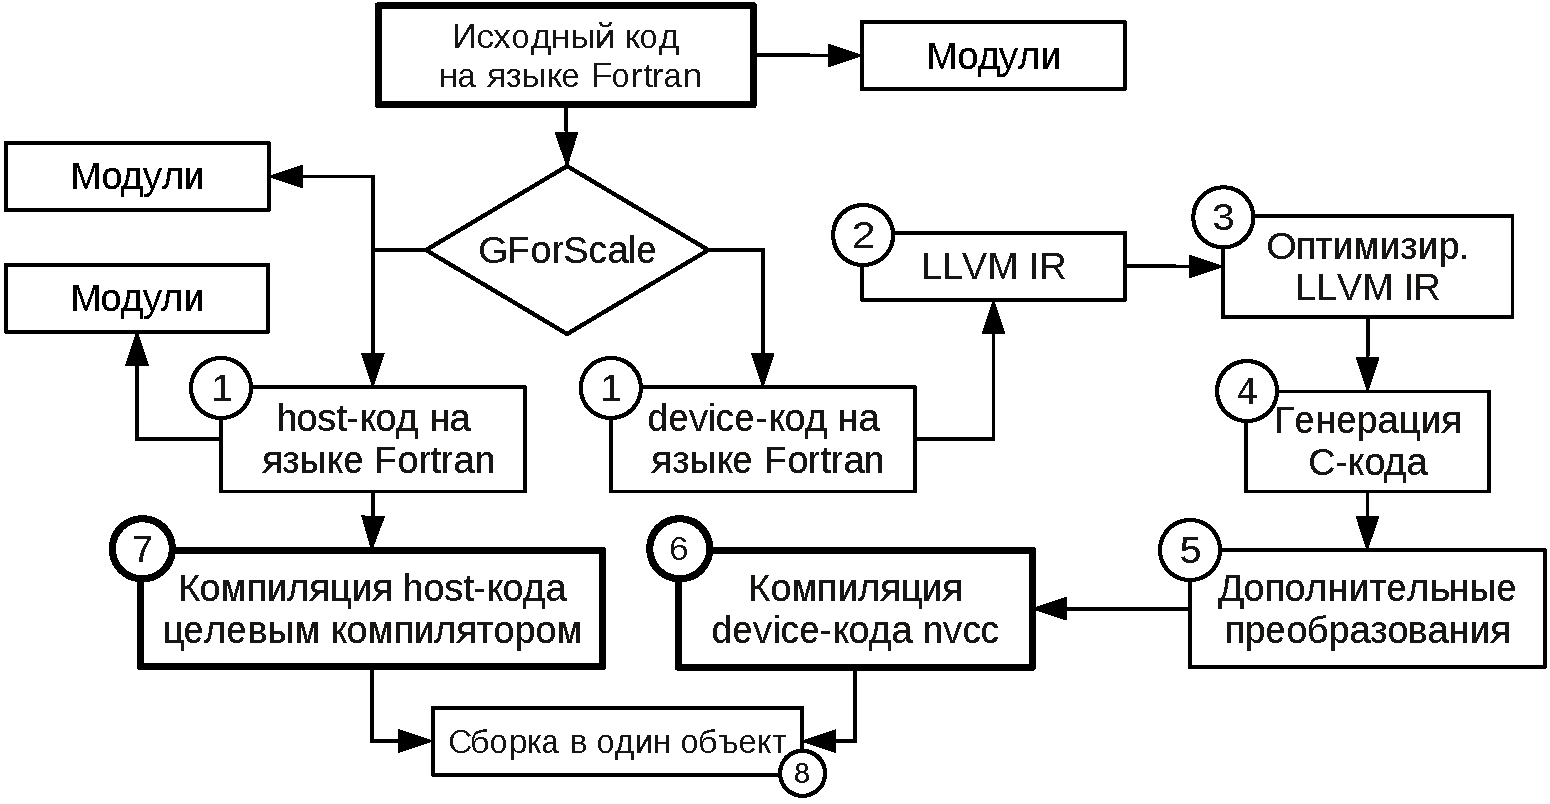
\includegraphics[scale=0.5]{figures/toolchain_scheme}
\caption{Общая схема генератора}
\label{fig:toolchain_scheme}
\end{figure}

\begin{enumerate}

\item

\begin{code}
/opt/kgen/bin/kgen-gforscale
-Wk,--gforscale-scene-path=/opt/kgen/transforms/split/
-Wk,--gforscale-specific-mode=default
-Wk,--gforscale-markup-mode=tree -g -c axpy.f90 -D__CUDA_DEVICE_FUNC__
\end{code}

Из обычного исходного кода на языке Fortran генерируются части эквивалентного кода на языках Fortran и C++ (части на C++ являются вспомогательными). Одни части кода подлежат исполнению на CPU, другие - на GPU. Разделение кода на части производит скрипт kgen-gforscale, используя преобразования внутреннего XML-представления исходного кода.

\begin{code}
/opt/llvm/dragonegg/bin/dragonegg-gfortran -g -c axpy.host.F90
-D__CUDA_DEVICE_FUNC__ -ffree-line-length-none -I/opt/kgen/include -o
axpy.host.F90.o
\end{code}

Перед следующим шагом часть кода для CPU проходит через компилятор \emph{/opt/llvm/dragonegg/bin/dragonegg-gfortran} для получения mod-файлов соответствующей версии. Они необходимы, так как содержат используемую Fortran-фронтендом информацию о данных, совместно используемых несколькими объектами. Формат mod-файлов слабо стандартизирован, поэтому они должны точно соответствовать компилятору.
\item

\begin{code}
/opt/llvm/dragonegg/bin/dragonegg-gfortran -c
axpy.axpy_loop_1_gforscale.device.F90 -D__CUDA_DEVICE_FUNC__
-ffree-line-length-none
-fplugin=/opt/llvm/dragonegg/lib64/dragonegg.so -O0 -S
-fplugin-arg-dragonegg-emit-ir -o axpy.axpy_loop_1_gforscale.device.F90.bc
\end{code}

Части исходного кода на языке Fortran, предназначенные для GPU преобразуются в LLVM IR (Low Level Virtual Machine Intermediate Representation) c помощью компилятора gfortran и плагина dragonegg.

\item

\begin{code}
/opt/llvm/bin/opt -std-compile-opts
axpy.axpy_loop_1_gforscale.device.F90.bc -S -o
axpy.axpy_loop_1_gforscale.device.F90.bc.opt
\end{code}

Оптимизирующий проход LLVM, благодаря которому генерируемый на
следующем шаге CUDA-код становится более эффективным и удобным для чтения.
Процессы анализа и оптимизации IR-кода в LLVM состоят из проходов (passes),
анализирующих или трансформирующих код (т.е. получающих новую версию IR).

\item

\begin{code}
/opt/llvm/bin/llc -march=c axpy.axpy_loop_1_gforscale.device.F90.bc.opt
-o axpy.axpy_loop_1_gforscale.device.F90.bc.cu
\end{code}

Генерация CUDA-кода из LLVM IR с помощью модифицированного LLVM C-Backend (файл \emph{llvm/lib/Target/CBackend/CBackend.cpp}).

\item Поиск и замена фрагментов исходного кода с подстановкой аттрибута \_\_global\_\_ в определение основной функции-ядра и реализаций \_\_device\_\_-функций, отображающих индексы циклов на индексы блоков GPU. Этот шаг не имеет специальной команды, его выполняет скрипт kgen с помощью регулярных выражений.

\begin{code}
$code =~ s/\#ifdef\s__CUDA_DEVICE_FUNC__\n__device__\n#endif\n
	void\s$name\_\(/#ifdef__CUDA_DEVICE_FUNC__\nextern "C" 
	__global__\n#endif\n#define $name\_$name\nvoid $name\_(/s;

$code =~ s/void\s$name\_blockidx_x\(unsigned\sint\s\*,\sunsigned\sint\s,
	\sunsignedint\s\)\;/void $name\_blockidx_x(unsigned int* index,
	unsigned int start, unsigned int end)
		{ *index = blockIdx.x + start; }/s;

$code =~ s/void\s$name\_blockidx_y\(unsigned\sint\s\*,\sunsigned\sint\s,
	\sunsigned int\s\)\;/void $name\_blockidx_y(unsigned int* index,
	unsigned int start, unsigned int end)
		{ *index = blockIdx.y + start; }/s;

$code =~ s/void\s$name\_blockidx_z\(unsigned\sint\s\*,\sunsigned\sint\s,
	\sunsigned int\s\)\;/void $name\_blockidx_z(unsigned int* index,
	unsigned int start, unsigned int end)
		{ *index = threadIdx.z + start; }/s;
\end{code}

\item

\begin{code}
nvcc -g -c axpy.axpy_loop_1_gforscale.device.F90.bc.cu 
-D__CUDA_DEVICE_FUNC__ --ptxas-options="-v" -arch=sm_20 -o
axpy.axpy_loop_1_gforscale.device.F90.o
\end{code}

Сборка части кода для GPU с помощью компилятора CUDA.

\item

\begin{code}
gfortran -g -c axpy.host.F90 -D__CUDA_DEVICE_FUNC__
-ffree-line-length-none -I/opt/kgen/include -o axpy.host.F90.o

gfortran -g -c axpy.axpy_loop_1_gforscale.host.F90
-D__CUDA_DEVICE_FUNC__ -ffree-line-length-none -I/opt/kgen/include -o
axpy.axpy_loop_1_gforscale.host.F90.o

g++ -g -I/opt/kgen/include -c axpy.axpy_loop_1_gforscale.host.cpp -o
axpy.axpy_loop_1_gforscale.host.cpp.o
\end{code}

Сборка частей кода для CPU - основного и вспомогательных объектов.

\item

\begin{code}
ld --unresolved-symbols=ignore-all -r -o axpy.o_kgen axpy.host.F90.o
axpy.axpy_loop_1_gforscale.host.F90.o
axpy.axpy_loop_1_gforscale.host.cpp.o
axpy.axpy_loop_1_gforscale.device.F90.o
\end{code}

Сборка объектов, соответствующих различным частям кода в единый объектный файл. За счёт этого результат работы генератора с точки зрения компоновки программных единиц идентичен обычному компилятору.

\item

\begin{code}
objcopy --wildcard
--localize-symbol=*__device_stub__*
--localize-symbol=*_gforscale_blockidx_*
--localize-symbol=*_gforscale_threadidx_*
--localize-symbol=*_gforscale_desc_*
--localize-symbol=*_gforscale_init*
--localize-symbol=*_gforscale_free*
--localize-symbol=*_loop_*_gforscale
--localize-symbol=*_gforscale_compare_ axpy.o_kgen axpy.o
\end{code}

Окончательная генерация результирующего объектного файла с переводом автоматически созданных функций в локальную область видимости для устранения потенциальных конфликтов имён на этапе линковки. Вместе с этим происходит перезапись объекта ранее созданного обычным компилятором, который был бы использован в случае, если генерация GPU-ядер по какой-либо причине не отработала корректно.

\end{enumerate}

\chapter{Генерация GPU-кода для модели COSMO}

ФФ

\chapter{Руководство пользователя}

Генератор GPU-ядер называется kgen-gfortran и в целом ведёт себя как обычный компилятор программ на языке Fortran, работать с ним столь же просто. Необходимые программы установлены на GPU-сервере СибНИГМИ и готовы к использованию. В данном разделе содержится описание опций компилятора и настроек среды, приведены примеры использования системы для компиляции моделей COSMO и WRF.

\section{Опции компилятора}

Компилятор kgen-gfortran вводит ряд дополнительных опций с префиксом -Wk для управления генерацией кода на GPU:

\vspace{15pt}
\begin{tabular}[h]{|l|l|p{7cm}|}
\hline
Опция & Значение & Комментарий \\ \hline \hline
-Wk,-\--bypass & --- & Отключение генерации GPU-ядер (компиляция только для CPU) \\ \hline
-Wk,-\--host-compiler= & gfortran & Имя внешнего компилятора для кода на CPU \\ \hline
-Wk,-\--kernel-compiler= & nvcc & Имя внешнего компилятора для GPU-ядер \\ \hline
-Wk,-\--kernel-target= & cuda & Программная модель для GPU \\ \hline
-Wk,-\--specific-mode= & cosmo & Специальный режим для компиляции определённой программы (эта опция будет удалена после добавления поддержки Polly) \\ \hline
\end{tabular}

\section{Настройка среды}

Компилятор kgen-gfortran обычно устанавливается в папку \emph{/opt/kgen/bin}, программы собранные с его помощью зависят от динамической библиотеки из \emph{/opt/kgen/lib/}. Подключить эти пути можно соответственно через переменные окружения PATH и LD\_LIBRARY\_PATH:

\begin{code}
$ export PATH=$PATH:/opt/kgen/bin
$ export LD_LIBRARY_PATH=$LD_LIBRARY_PATH:/opt/kgen/lib
\end{code}

Поведение программы, собранной kgen-gfortran можно настроить с помощью следующих переменных среды:

\vspace{15pt}
\begin{tabular}[h]{|l|l|p{7cm}|}
\hline
Переменная & Значение & Комментарий \\ \hline \hline
gforscale\_runmode & 1, 2, 3 & Режим исполнения для всех циклов: 1 - на CPU (по умолчанию), 2 - на GPU с поддержкой CUDA, 3 - и на CPU, и на CUDA GPU + сравнение результатов \\ \hline
gforscale\_debug\_output & 0, 1, 2, 3 & Отладочный вывод из функций runtime-библиотеки (по умолчанию 0 - отключён) \\ \hline
gforscale\_error\_output & 0, 1, 2, 3 & Вывод ошибок из функций runtime-библиотеки (по умолчанию \~0 - всё включено) \\ \hline
\%s\_loop\_\%d\_gforscale & 1, 2, 3 & Режим исполнения конкретного цикла с номером \%d в функции \%s: 1 - на CPU (по умолчанию), 2 - на GPU с поддержкой CUDA, 3 - и на CPU, и на CUDA GPU + сравнение результатов \\ \hline
\end{tabular}

\section{Компиляция COSMO}

\begin{code}
svn co file:///svn/cosmo
\end{code}

Переместившись в папку с исходным кодом компонентов модели, необходимо запустить make-скрипт с указанием флагов, подключающих генерацию GPU-ядер:

\begin{code}
cd cosmo/source
make HAVE_KERNELGEN=1 HAVE_KERNELGEN_CUDA=1
\end{code}

Обычно компиляция занимает продолжительное время. Если на системе доступно N > 1 ядер, то сборку можно ускорить за счёт параллельной компиляции добавлением опции -jN.

\section{Компиляция WRF}

Репозиторий с исходным кодом модели WRF версии 3.3 находится на GPU-сервере СибНИГМИ. По сравнению с официальным релизом, в нём сделано одно исправление, также kgen-gfortran добавлен в список поддерживаемых компиляторов. Любой пользователь системы может сделать локальную копию репозитория:

\begin{code}
svn co file:///svn/wrf
\end{code}

Переместившись в корневую папку файлов модели, необходимо запустить скрипт конфигурации с указанием пути к библиотекам NetCDF:

\begin{code}
cd wrf/
NETCDF=/opt/openmpi_kgen-1.4.4/ ./configure
\end{code}

Диалог выбора конфигурации будет содержать варианты сборки с использованием kgen-gfortran:

\begin{code}
  19.  Linux x86_64, kgen-gfortran generator for CUDA with gcc   (serial)
  20.  Linux x86_64, kgen-gfortran generator for CUDA with gcc   (smpar)
  21.  Linux x86_64, kgen-gfortran generator for CUDA with gcc   (dmpar)
  22.  Linux x86_64, kgen-gfortran generator for CUDA with gcc   (dm+sm)
\end{code}

Далее сборка производится скриптом ./compile с указанием одной из предопределённых конфигураций модели:

\begin{code}
./compile em_tropical_cyclone
\end{code}

Обычно компиляция занимает продолжительное время. Если на системе доступно N > 1 ядер, то сборку можно ускорить за счёт параллельной компиляции добавлением опции -jN.

\section{Ограничения}

Компилятор kgen-gfortran может быть недостаточно хорошо совместим с некоторыми сложными configure-скриптами. При необходимости выполнения configure-скрипта следует переключить значение переменной bypass в файле \emph{/opt/kgen/bin/kgen} на 1, а после завершения конфигурации --- вернуть обратно 0.

\chapter{Дополнительные сведения для разработчиков}

\section{Компиляция компонентов системы}

ФФ

\subsection{LLVM}

Загрузка исходного кода (последняя протестированная ревизия --- 134365):

\begin{code}
svn co http://llvm.org/svn/llvm-project/llvm/trunk llvm -r134365
cd llvm/
\end{code}

Наложение двух патчей, исправляющих две открытые проблемы LLVM C-backend и третьего --- для обеспечения генерации CUDA-кода.

\begin{code}
patch -d . -p1 < ../kernelgen/patches/llvm/varargs.patch 
patch -d . -p1 < ../kernelgen/patches/llvm/inlasm.patch
patch -d . -p1 < ../kernelgen/patches/llvm/nvcc.patch 
\end{code}

Сборка и установка LLVM:

\begin{code}
mkdir build
cp -rf include/ build/include/
cd build
../configure --enable-jit --enable-optimized --enable-shared --prefix=/opt/llvm
--enable-targets=host,cbe
make -j12 CXXFLAGS=-O3
sudo make install
\end{code}

В опциях указан путь для установки \emph{/opt/llvm} и поддержка архитектур host (архитектура данной машины) и cbe (C backend).

Добавить llvm в пути можно стандартным образом --- через PATH и LD\_LIBRARY\_PATH или /etc/profile.d/ и /etc/ld.so.conf.d/:

\begin{code}
export LD_LIBRARY_PATH=$LD_LIBRARY_PATH:/opt/llvm/lib:/opt/llvm/lib64/
export PATH=$PATH:/opt/llvm/bin
\end{code}

\begin{code}
$cat /etc/ld.so.conf.d/llvm.conf 
/opt/llvm/lib
$cat /etc/profile.d/llvm.sh 
export PATH=$PATH:/opt/llvm/bin
\end{code}

\subsection{GNU GCC 4.5}

Зависимости для системы Fedora:
\begin{itemize}
\item gmp-devel, mpfr-devel, libmpc-devel
\item elfutils-libelf-devel
\item flex
\item glibc-devel.i686
\end{itemize}


Зависимости для системы Debian / Ubuntu:
\begin{itemize}
\item libgmp3-dev, libmpfr-dev, libmpc-dev
\item libelf-dev
\item flex
\item libc6-dev, libc6-dev-i386
\item gcc-multilib
\end{itemize}

Загрузка исходного кода (последняя протестированная ревизия --- 174313), cборка и установка:

\begin{code}
svn co http://llvm.org/svn/llvm-project/dragonegg/trunk dragonegg
svn co http://gcc.gnu.org/svn/gcc/branches/gcc-4_5-branch gcc-4.5 -r174313
cd gcc-4.5/
patch -d . -p1 < ../kernelgen/patches/gcc/gcc.patch
mkdir build
cd build/
../configure --prefix=/opt/llvm/dragonegg/ --program-prefix=dragonegg-
--enable-languages=c,c++,fortran --with-mpfr-include=/usr/include/
--with-mpfr-lib=/usr/lib64 --with-gmp-include=/usr/include/
--with-gmp-lib=/usr/lib64 --enable-plugin
make -j12
sudo make install
\end{code}

\section{DragonEgg}

\begin{comment}
Now compile llvm as gcc plugin:

{{{
cd dragonegg/
GCC=/opt/llvm/dragonegg/bin/dragonegg-gcc LLVM_CONFIG=/opt/llvm/bin/llvm-config make
sudo cp dragonegg.so /opt/llvm/dragonegg/lib64/
}}}

= LLVM with C backend pass and GPU kernels generation (KGEN) =

This version of toolkit alters the usual compilation pipeline by adding C code generation step between translation to IR and target assembly and transforms computational loops to GPU kernels. In other words, straight-forward compiler pipeline usually looks like:

{{{
source code -> AST / LLVM IR -> assembly
}}}

In contrast, ''LLVM with CBE backend pass'' stands for:

{{{
source code -> LLVM IR -> C code -> GPU kernels -> mixed host & GPU assembly
}}}

Construction of reliable compilation pipeline with intermediate C code generation is a major milestone in our project. It enables offloading parts of original code (in any frontend-supported language) onto accelerators in C code. Having C code on device is the easiest way to accomplish the whole thing, since we don't need to deal with buggy toolchains from 3rd party trolls.

The toolchain implementing the modified compilation pipeline showed above is prefixed '''kgen'''-*. It consists of a set of wrappers (Perl scripts) on top of the gcc 4.5 compiler with dragonegg plugin.

'''Prerequisites''' (names for packages in Fedora repos)
 * perl-XML-LibXSLT
 * perl-IPC-Run3
 * libffi-devel
 * gcc-gfortran

'''Prerequisites''' (names for packages in Debian / Ubuntu repos)
 * libxml-xslt-perl
 * libipc-run3-perl
 * libffi-dev
 * gfortran

Sources can be found in ''kernelgen/src''. Preconfigured environment and test cases can be evaluated on our [https://tesla.parallel.ru/trac/kernelgen/wiki/TestServer test server]. Toolchain can be built and installed easily:

{{{
cd kernelgen/src
make
sudo make install
}}}

Add /opt/kgen/bin into your $PATH and /opt/kgen/lib into LD_LIBRARY_PATH.

'''NOTE:''' if you're using GPU older than sm_20, please edit /opt/kgen/bin/kgen and comment out -arch=sm_20 option or replace it with your best capability.

= Running KGen builtin public test suite =

The purpose of public test suite is to check various simple apps utilizing different Fortran features are working correctly.

Compile:

{{{
...
[marcusmae@noisy kernelgen]$ cd tests/
[marcusmae@noisy tests]$ make
cd public/axpy && make
make[1]: Entering directory `/home/marcusmae/Programming/kernelgen/tests/public/axpy'
kgen-gfortran -Wk,--kernel-compiler=nvcc -Wk,--kernel-target=cuda -g -c axpy.f90 -o axpy.o
/opt/kgen/bin/kgen-gforscale -Wk,--gforscale-scene-path=/opt/kgen/transforms/split/ -Wk,--gforscale-specific-mode=default -Wk,--gforscale-markup-mode=tree axpy.f90
gforscale       >> axpy.f90:16: portable 1-dimensional loop
gforscale       >> axpy.f90:16: selecting this loop
/opt/llvm/dragonegg/bin/dragonegg-gfortran -g -c axpy.host.F90 -D__CUDA_DEVICE_FUNC__ -ffree-line-length-none -I/opt/kgen/include -o axpy.host.F90.o
gfortran -g -c axpy.axpy_loop_1_gforscale.host.F90 -D__CUDA_DEVICE_FUNC__ -ffree-line-length-none -I/opt/kgen/include -o axpy.axpy_loop_1_gforscale.host.F90.o
/opt/llvm/dragonegg/bin/dragonegg-gfortran -c axpy.axpy_loop_1_gforscale.device.F90 -D__CUDA_DEVICE_FUNC__ -ffree-line-length-none -fplugin=/opt/llvm/dragonegg/lib64/dragonegg.so -O0 -S -fplugin-arg-dragonegg-emit-ir -o axpy.axpy_loop_1_gforscale.device.F90.bc
/opt/llvm/bin/opt -std-compile-opts axpy.axpy_loop_1_gforscale.device.F90.bc -S -o axpy.axpy_loop_1_gforscale.device.F90.bc.opt
/opt/llvm/bin/llc -march=c axpy.axpy_loop_1_gforscale.device.F90.bc.opt -o axpy.axpy_loop_1_gforscale.device.F90.bc.cu
nvcc -g -c axpy.axpy_loop_1_gforscale.device.F90.bc.cu -D__CUDA_DEVICE_FUNC__ -G --ptxas-options="-v" -arch=sm_20 -o axpy.axpy_loop_1_gforscale.device.F90.o
c       >> ptxas info    : Compiling entry function 'axpy_loop_1_gforscale_' for 'sm_20'
c       >> ptxas info    : Function properties for axpy_loop_1_gforscale_                                                                                
c       >>     8 bytes stack frame, 0 bytes spill stores, 0 bytes spill loads                                                                            
c       >> ptxas info    : Function properties for _Z32axpy_loop_1_gforscale_blockidx_xPjjj                                                              
c       >>     0 bytes stack frame, 0 bytes spill stores, 0 bytes spill loads                                                                            
c       >> ptxas info    : Used 13 registers, 64 bytes cmem[0]                                                                                           
gfortran -g -c axpy.host.F90 -D__CUDA_DEVICE_FUNC__ -ffree-line-length-none -I/opt/kgen/include -o axpy.host.F90.o                                       
ld --unresolved-symbols=ignore-all -r -o axpy.o_kgen axpy.host.F90.o axpy.axpy_loop_1_gforscale.host.F90.o axpy.axpy_loop_1_gforscale.device.F90.o       
mv axpy.o_kgen axpy.o                                                                                                                                    
gcc -g -std=c99 -I/opt/kgen/include -c main.c -o main.o                                                                                                  
kgen-gfortran -Wk,--kernel-compiler=nvcc -Wk,--kernel-target=cuda main.o axpy.o -o axpy
make[1]: Leaving directory `/home/marcusmae/Programming/kernelgen/tests/public/axpy'
cd public/logexp && make
make[1]: Entering directory `/home/marcusmae/Programming/kernelgen/tests/public/logexp'
kgen-gfortran -Wk,--kernel-compiler=nvcc -Wk,--kernel-target=cuda -g -c logexp.f90 -o logexp.o
/opt/kgen/bin/kgen-gforscale -Wk,--gforscale-scene-path=/opt/kgen/transforms/split/ -Wk,--gforscale-specific-mode=default -Wk,--gforscale-markup-mode=tree logexp.f90                                                                                                                                             
gforscale       >> logexp.f90:39: portable 2-dimensional loop                                                                                            
gforscale       >> logexp.f90:39: selecting this loop                                                                                                    
/opt/llvm/dragonegg/bin/dragonegg-gfortran -g -c logexp.host.F90 -D__CUDA_DEVICE_FUNC__ -ffree-line-length-none -I/opt/kgen/include -o logexp.host.F90.o 
gfortran -g -c logexp.logexp_loop_1_gforscale.host.F90 -D__CUDA_DEVICE_FUNC__ -ffree-line-length-none -I/opt/kgen/include -o logexp.logexp_loop_1_gforscale.host.F90.o                                                                                                                                            
/opt/llvm/dragonegg/bin/dragonegg-gfortran -c logexp.logexp_loop_1_gforscale.device.F90 -D__CUDA_DEVICE_FUNC__ -ffree-line-length-none -fplugin=/opt/llvm/dragonegg/lib64/dragonegg.so -O0 -S -fplugin-arg-dragonegg-emit-ir -o logexp.logexp_loop_1_gforscale.device.F90.bc                                      
/opt/llvm/bin/opt -std-compile-opts logexp.logexp_loop_1_gforscale.device.F90.bc -S -o logexp.logexp_loop_1_gforscale.device.F90.bc.opt                  
/opt/llvm/bin/llc -march=c logexp.logexp_loop_1_gforscale.device.F90.bc.opt -o logexp.logexp_loop_1_gforscale.device.F90.bc.cu                           
nvcc -g -c logexp.logexp_loop_1_gforscale.device.F90.bc.cu -D__CUDA_DEVICE_FUNC__ -G --ptxas-options="-v" -arch=sm_20 -o logexp.logexp_loop_1_gforscale.device.F90.o                                                                                                                                              
                                                                                                                                                         
c       >> ptxas info    : Compiling entry function 'logexp_loop_1_gforscale_' for 'sm_20'
c       >> ptxas info    : Function properties for logexp_loop_1_gforscale_                                                                              
c       >>     8 bytes stack frame, 0 bytes spill stores, 0 bytes spill loads                                                                            
c       >> ptxas info    : Function properties for _Z34logexp_loop_1_gforscale_blockidx_xPjjj                                                            
c       >>     0 bytes stack frame, 0 bytes spill stores, 0 bytes spill loads                                                                            
c       >> ptxas info    : Function properties for _Z34logexp_loop_1_gforscale_blockidx_yPjjj                                                            
c       >>     0 bytes stack frame, 0 bytes spill stores, 0 bytes spill loads                                                                            
c       >> ptxas info    : Used 18 registers, 72 bytes cmem[0]                                                                                           
gfortran -g -c logexp.host.F90 -D__CUDA_DEVICE_FUNC__ -ffree-line-length-none -I/opt/kgen/include -o logexp.host.F90.o                                   
ld --unresolved-symbols=ignore-all -r -o logexp.o_kgen logexp.host.F90.o logexp.logexp_loop_1_gforscale.host.F90.o logexp.logexp_loop_1_gforscale.device.F90.o                                                                                                                                                    
mv logexp.o_kgen logexp.o                                                                                                                                
gcc -g -std=c99 -I/opt/kgen/include -c main.c -o main.o                                                                                                  
kgen-gfortran -Wk,--kernel-compiler=nvcc -Wk,--kernel-target=cuda main.o logexp.o -o logexp
make[1]: Leaving directory `/home/marcusmae/Programming/kernelgen/tests/public/logexp'
...
}}}

Run:

{{{
...
marcusmae@noisy tests]$ make tests
./runtests
sizeof(LOGICAL) = 4
sizeof(LOGICAL) = 4
[  OK  ] public/szlogical/szlogical
arg "unknown" ref = 0x7ffff5d26e28, size = 4, desc = 0x7ffff5d26e28
arg "unknown" ref = 0x7ffff5d26e28, size = 4 duplicated to 0x925ca0 for results comparison
arg "unknown" ref = 0x911140, size = 40, desc = 0x911140
arg "unknown" ref = 0x911140, size = 40 duplicated to 0x925ce0 for results comparison
arg "unknown" ref = 0x7ffff5d26e24, size = 4, desc = 0x7ffff5d26e24
arg "unknown" ref = 0x7ffff5d26e24, size = 4 duplicated to 0x925d30 for results comparison
arg "unknown" ref = 0x911110, size = 40, desc = 0x911110
arg "unknown" ref = 0x911110, size = 40 duplicated to 0x925d70 for results comparison
symbol "unknown" maps memory segment [0x925ca0 .. 0x925ca4] to [0x200100ca0 .. 0x200100ca4]
symbol "unknown" maps memory segment [0x925ce0 .. 0x925d08] to [0x200120ce0 .. 0x200120d08]
symbol "unknown" maps memory segment [0x925d30 .. 0x925d34] to [0x200140d30 .. 0x200140d34]
symbol "unknown" maps memory segment [0x925d70 .. 0x925d98] to [0x200160d70 .. 0x200160d98]
 Value of i after cycle =           11
[  OK  ] axpy_1=2 public/axpy/axpy 10
arg "unknown" ref = 0x7fff37b468e8, size = 4, desc = 0x7fff37b468e8
arg "unknown" ref = 0x7fff37b468e8, size = 4 duplicated to 0x1897ba0 for results comparison
arg "unknown" ref = 0x18820c0, size = 4000, desc = 0x18820c0
arg "unknown" ref = 0x18820c0, size = 4000 duplicated to 0x1897be0 for results comparison
arg "unknown" ref = 0x7fff37b468e4, size = 4, desc = 0x7fff37b468e4
arg "unknown" ref = 0x7fff37b468e4, size = 4 duplicated to 0x1898bb0 for results comparison
arg "unknown" ref = 0x1881110, size = 4000, desc = 0x1881110
arg "unknown" ref = 0x1881110, size = 4000 duplicated to 0x1898bf0 for results comparison
symbol "unknown" maps memory segment [0x1897ba0 .. 0x1897ba4] to [0x200100ba0 .. 0x200100ba4]
symbol "unknown" maps memory segment [0x1897be0 .. 0x1898b80] to [0x200120be0 .. 0x200121b80]
symbol "unknown" maps memory segment [0x1898bb0 .. 0x1898bb4] to [0x200140bb0 .. 0x200140bb4]
symbol "unknown" maps memory segment [0x1898bf0 .. 0x1899b90] to [0x200160bf0 .. 0x200161b90]
 Value of i after cycle =         1001
[  OK  ] axpy_1=2 public/axpy/axpy 1000
arg "unknown" ref = 0x7fff96039d6c, size = 4, desc = 0x7fff96039d6c
arg "unknown" ref = 0x7fff96039d6c, size = 4 duplicated to 0x22b11f0 for results comparison
arg "unknown" ref = 0x7fff96039d70, size = 4, desc = 0x7fff96039d70
arg "unknown" ref = 0x7fff96039d70, size = 4 duplicated to 0x22b1230 for results comparison
arg "unknown" ref = 0x229c450, size = 400, desc = 0x229c450
arg "unknown" ref = 0x229c450, size = 400 duplicated to 0x22b1270 for results comparison
arg "unknown" ref = 0x229c110, size = 400, desc = 0x229c110
arg "unknown" ref = 0x229c110, size = 400 duplicated to 0x22b1430 for results comparison
arg "unknown" ref = 0x229c2b0, size = 400, desc = 0x229c2b0
arg "unknown" ref = 0x229c2b0, size = 400 duplicated to 0x22b15f0 for results comparison
symbol "unknown" maps memory segment [0x22b11f0 .. 0x22b11f4] to [0x2001001f0 .. 0x2001001f4]
symbol "unknown" maps memory segment [0x22b1230 .. 0x22b1234] to [0x200120230 .. 0x200120234]
symbol "unknown" maps memory segment [0x22b1270 .. 0x22b1400] to [0x200140270 .. 0x200140400]
symbol "unknown" maps memory segment [0x22b1430 .. 0x22b15c0] to [0x200160430 .. 0x2001605c0]
symbol "unknown" maps memory segment [0x22b15f0 .. 0x22b1780] to [0x2001805f0 .. 0x200180780]
 Value of i after cycle =           11
 Value of j after cycle =           11
[  OK  ] logexp_1=2 public/logexp/logexp 10 10
...
}}}

= OpenMPI for KGen =

'''NOTE:''' This step is useful only if you plan to use kgen-gfortran integrated into OpenMPI, i.e. if your program utilizes Message Passing Interface (MPI). It is not always the case and could be skipped.

{{{
wget http://www.open-mpi.org/software/ompi/v1.5/downloads/openmpi-1.5.3.tar.bz2
tar -xjf openmpi-1.5.3.tar.bz2
cd openmpi-1.5.3
}}}

Before configuring, change '''bypass''' flag in /opt/kgen/bin/kgen to 2 and set it back to 0 after configuring.

{{{
mkdir build
cd build
../configure --prefix=/opt/openmpi_kgen-1.5.3 CC=gcc CXX=g++ F77="/opt/kgen/bin/kgen-gfortran" FC="/opt/kgen/bin/kgen-gfortran"
make -j12
make install
}}}

Note absolute compiler paths - they may be required to workaround the stupid problems during installing: scripts cannot find compilers otherwise.

Place mpivars.sh and mpivars.csh into /opt/openmpi_kgen-1.5.3/etc folder:

{{{
[dmikushin@tesla-cmc ~]$ cat /opt/openmpi_kgen-1.5.3/etc/mpivars.sh
# PATH
if test -z "`echo $PATH | grep /opt/openmpi_kgen-1.5.3/bin`"; then
    PATH=/opt/openmpi_kgen-1.5.3/bin:${PATH}
    export PATH
fi

# LD_LIBRARY_PATH
if test -z "`echo $LD_LIBRARY_PATH | grep /opt/openmpi_kgen-1.5.3/lib`"; then
    LD_LIBRARY_PATH=/opt/openmpi_kgen-1.5.3/lib${LD_LIBRARY_PATH:+:}${LD_LIBRARY_PATH}
    export LD_LIBRARY_PATH
fi

# MANPATH
if test -z "`echo $MANPATH | grep /opt/openmpi_kgen-1.5.3/share/man`"; then
    MANPATH=/opt/openmpi_kgen-1.5.3/share/man:${MANPATH}
    export MANPATH
fi
}}}

{{{
[dmikushin@tesla-cmc ~]$ cat /opt/openmpi_kgen-1.5.3/etc/mpivars.csh
# PATH
if ("" == "`echo $path | grep /opt/openmpi_kgen-1.5.3/bin`") then
    set path=(/opt/openmpi_kgen-1.5.3/bin $path)
endif

# LD_LIBRARY_PATH
if ("1" == "$?LD_LIBRARY_PATH") then
    if ("$LD_LIBRARY_PATH" !~ */opt/openmpi_kgen-1.5.3/lib*) then
        setenv LD_LIBRARY_PATH /opt/openmpi_kgen-1.5.3/lib:${LD_LIBRARY_PATH}
    endif
else
    setenv LD_LIBRARY_PATH /opt/openmpi_kgen-1.5.3/lib
endif

# MANPATH
if ("1" == "$?MANPATH") then
    if ("$MANPATH" !~ */opt/openmpi_kgen-1.5.3/share/man*) then
        setenv MANPATH /opt/openmpi_kgen-1.5.3/share/man:${MANPATH}
    endif
else
    setenv MANPATH /opt/openmpi_dragonegg-1.5.3/share/man:
endif
}}}

Register OpenMPI implementation with mpi-selector table:

{{{
mpi-selector --register openmpi_kgen-1.5.3 --source-dir /opt/openmpi_kgen-1.5.3/etc/
}}}
\end{comment}


\chapter{Лицензионный статус}

Реализация, полученная в данном проекте является надстройкой над множеством различных программ. В данном разделе собраны сведения о лицензионном статусе используемых компонентов. Все они так или иначе доступны в исходных кодах, за исключением части cuda toolkit.

\vspace{15pt}
\begin{tabular}[h]{|l|l|p{9cm}|}
\hline
Название & Лицензия & Комментарий \\ \hline \hline
llvm & BSD & Инфраструктура компилятора LLVM \\ \hline
gfortran & GPL & Компилятор GNU Fortran \\ \hline
dragonegg & BSD & Плагин, связывающий llvm и gfortran \\ \hline
g95 & GPL & Компилятор Fortran \\ \hline
g95xml & GPL & XML-разметка исходного кода на основе компилятора g95 \\ \hline
libxml/libxslt & MIT & Библиотека для работы c XML и XSLT \\ \hline
nvopencc & GPL & Вариант компилятора open64 с поддержой генерации GPU-ядер на CUDA \\ \hline
cuda toolkit & NVIDIA & Инфраструктура компилятора NVIDIA CUDA \\ \hline
\end{tabular}

\chapter{План развития}

В этом разделе дано описание конкретных технических подзадач, соответствующих общему плану работ.

\section{Первый этап (окончен)}

\begin{enumerate}
\item Реализация программы-драйвера по типу gcc или nvcc, организующей запуск приложений, ответственных за отдельные этапы компиляции
\item Тестирование генерации кода на CUDA С с помощью LLVM C Backend, обсуждение существенных проблем с разработчиками LLVM, написание патчей
\item Доработка созданной в 2009 г. системы расщепления исходного кода на части для CPU и GPU на основе g95-xml
\item Разработка runtime-библиотеки:
\begin{enumerate}
\item Запуск ядер и упаковка аргументов с помощью CUDA API
\item Синхронизация данных двумя способами: явно (cudaMalloc/cudaMemcpy) и memory mapping (zero-copy)
\item Поддежрка синхронизации allocatable-переменных и данных в модулях
\end{enumerate}
\item Разработка системы контроля правильности результатов на уровне отдельных ядер:
\begin{enumerate}
\item Запуск ядра с предварительной дубликацией входных и выходных данных
\item Генерация функции сравнения результатов для каждого ядра
\end{enumerate}
\item Сборка модели COSMO с помощью генератора, представление результатов корректной работы большого множества GPU-ядер
\item Реализация набора базовых тестов для автоматизированного контроля регрессивных изменений
\end{enumerate}

\section{Второй этап}

\begin{enumerate}
\item Улучшение поддержки/совместимости генератора с различными моделями
\item Улучшение производительности/эффективности
\item Сравнение производительности с другими системами и результатами проектов POMPA
\end{enumerate}

\subsection{Задачи поддержки/совместимости}

\begin{enumerate}
\item Тестирование сборки COSMO и других моделей конечными пользователями, отчёты об ошибках (участники от СибНИГМИ)
\begin{enumerate}
\item Проверка сборки рабочей версии модели WRF с помощью kgen-gfortran
\item Проверка сборки модели ПЛАВ, предварительное переключение на gcc, если текущая версия настроена на компилятор Intel (совместимость с Intel не тестировалась)
\end{enumerate}
\item Исправление наиболее существенных ошибок и недоработок в системе разделения кода
\begin{enumerate}
\item Решение проблем с использованием производных типов (структур)
\end{enumerate}
\item Использование Polly/Pluto для точного определения параллельных циклов
\begin{enumerate}
\item Освоение pluto и polly для LLVM на простых тестах
\item Проверка возможности добавления шага polly LLVM перед генерацией CUDA-кода
\item Освоение методов реконструкции данных о циклах из представления LLVM IR, проверка возможности получения этой информации после прохода polly и её использования в конфигурации грида GPU.
\end{enumerate}
\item Частичная докомпиляция ядер с внешними зависимостями на этапе линковки
\begin{enumerate}
\item Выбор метода поиска внешних зависимостей
\item Поддержка хранения метаданных в специальной секции объектных файлов
\item Реализация скрипта линковки kgen-ld с комбинированием исходного кода нескольких зависимых объектов в единый объект и перекомпиляцией
\end{enumerate}
\end{enumerate}

\subsection{Задачи производительности/эффективности}

\begin{enumerate}
\item Использование разделяемой памяти в шаблонах численных схем (Александр Мыльцев)
\begin{enumerate}
\item Изучение литературы по существующим генераторам на основе ROSE или Polly
\item Добавление простой реализации в преобразования XSLT
\end{enumerate}
\item Уменьшение времени запуска GPU-ядер (кеширование конфигураций)
\begin{enumerate}
\item Перенос определения статических зависимостей GPU-ядра в секцию инициализации
\item Решение проблем с использованием \_\_attribute\_\_(constructor) в CUDA или проработка обходного пути
\end{enumerate}
\item Уменьшение времени обмена данными
\begin{enumerate}
\item (вариант) Портирование на GPU также и последовательного кода в режиме одного потока (теоретически, значительно меньше обменов, остаётся только вывод и MPI)
\begin{enumerate}
\item Имеет смысл только при отличном качестве работы системы разделения кода
\item Установка device-заглушек на вызовы функций gfortran runtime library
\item Генерация GPU-ядер для последовательных циклов в режиме одного потока
\item Реализация некоторых функций gfortran runtime library для GPU (работа с памятью, печать, вывод)
\end{enumerate}
\item (вариант) Поддержка выборочной/отложенной синхронизации данных на основе статического графа зависимостей (гибкий вариант)
\begin{enumerate}
\item Подключение g95xml-refids в систему разделения кода, реализация правила статического поиска символов, зависящих от символов в ядре, установка точек обязательной синхронизации данных
\end{enumerate}
\end{enumerate}
\item (предложение С.~В.~Ковылова) Реализация гибридного разделения вычислений между CPU и GPU
\end{enumerate}

\section{Предложения координационного характера}

\begin{enumerate}
\item Организация официального хостинга проекта в СибНИГМИ, переезд проекта с tesla.parallel.ru (возможно, на sscc)
\item Согласование возможных вариантов тестирования multi-GPU режима (подача заявки на доступ к одному из GPU-кластеров МГУ, разрешение на тестирование в NVIDIA и др.)
\item Разрешение на контакт с участниками COSMO/POMPA с целью представления результатов на ближайшей встрече разработчиков (сентябрь 2011, Рим)
\end{enumerate}

\end{document}
